\documentclass{ieeeaccess}

\usepackage[utf8]{inputenc}
\usepackage[T1]{fontenc}
\usepackage{cite}
\usepackage{amsmath,amssymb,amsfonts}
\usepackage{algorithmic}
\usepackage{graphicx}
\usepackage{textcomp}
\usepackage{bm}
\usepackage{booktabs}
\usepackage{array}
\usepackage{adjustbox}
\usepackage{url}
\usepackage{float}
\usepackage{xcolor}
\usepackage[hidelinks]{hyperref}
\usepackage{placeins}
\usepackage{etoolbox}

\newcommand{\orcidid}[1]{%
  \href{https://orcid.org/#1}{
\includegraphics[width=9pt]{Orcid_icon.png}}%
}

\makeatletter
\AtBeginDocument{\DeclareMathVersion{bold}
\SetSymbolFont{operators}{bold}{T1}{times}{b}{n}
\SetSymbolFont{NewLetters}{bold}{T1}{times}{b}{it}
\SetMathAlphabet{\mathrm}{bold}{T1}{times}{b}{n}
\SetMathAlphabet{\mathit}{bold}{T1}{times}{b}{it}
\SetMathAlphabet{\mathbf}{bold}{T1}{times}{b}{n}
\SetMathAlphabet{\mathtt}{bold}{OT1}{pcr}{b}{n}
\SetSymbolFont{symbols}{bold}{OMS}{cmsy}{b}{n}
\renewcommand\boldmath{\@nomath\boldmath\mathversion{bold}}}
\makeatother

% Hide the DOI label when no DOI is assigned yet.
\makeatletter
\patchcmd{\@maketitle}{Digital Object Identifier\space\@doi}{}{}{}
\patchcmd{\@jtehmmaketitle}{Digital Object Identifier\space\@doi}{}{}{}
\patchcmd{\editorialmaketitle}{Digital Object Identifier\space\@doi}{}{}{}
% Hide the IEEE Access template volume/year footer without editing ieeeaccess.cls.
\def\footervolfont{\color{white}\fontsize{1}{1}\selectfont}
\makeatother

\def\BibTeX{{\rm B\kern-.05em{\sc i\kern-.025em b}\kern-.08em
    T\kern-.1667em\lower.7ex\hbox{E}\kern-.125emX}}


\begin{document}
\history{}
\doi{}

\title{A SaaS-IoT Architecture for Traceable Energy Performance Indicators and Preliminary Distributed Machine-Level Monitoring}

\author{
\uppercase{Andres Viveros}\,\orcidid{0000-0003-4917-6798}\authorrefmark{1,2},
\uppercase{Ivan Derpich}\,\orcidid{0000-0001-9759-7285}\authorrefmark{1,2},
\uppercase{Juan Miguel Sepúlveda}\,\orcidid{0000-0003-3755-0981}\authorrefmark{1,2}
}

\address[1]{Centre for Innovation in Technology and Design of Materials for the Built Environment (CIMAC), ANID CTI250005, Universidad de Santiago de Chile, Santiago, Chile}
\address[2]{Department of Industrial Engineering, Faculty of Engineering,
Universidad de Santiago de Chile, Santiago, Chile}

\tfootnote{This work was developed in the context of the EnPi project for industrial energy management and distributed energy performance monitoring.}

\markboth
{Viveros \headeretal: EnPi: SaaS-IoT Architecture for Traceable Energy Performance Indicators}
{Viveros \headeretal: EnPi: SaaS-IoT Architecture for Traceable Energy Performance Indicators}

\corresp{Corresponding author: Andres Viveros (e-mail: andres.viverosll@usach.cl).}

\begin{abstract}
Industrial energy management requires traceable information linking consumption, production, equipment, and processes to support operational control, evidence preparation, and energy performance indicators. This challenge is especially relevant for small and medium-sized enterprises, where cost, technical complexity, and data integration barriers hinder monitoring adoption. Although IoT meters, cyber-physical systems, and energy platforms have advanced, few solutions combine equipment-level metering, production records, traceability, and EnPI calculation within a progressive-adoption SaaS model. This article proposes EnPi, a modular SaaS-IoT architecture comprising a web platform, a traceable data model, and plug-and-play single-phase nodes. The contribution is positioned as an architectural and functional implementation with preliminary component-level validation, not as industrial-scale platform validation or metrological certification. EnPi integrates manual and IoT data, production records, target references, alert rules, and EnPI calculation as consumed energy per production unit. Validation used parallel measurements from an EnPi node and a calibrated Metrel MI2883 analyzer across ten load scenarios and 10,596 paired samples. An anonymized food-sector SME use case monitored a dough sheeter producing 44 kg per production day. Results showed high agreement in current, power factor, and voltage, with Pearson coefficients of 0.9998, 0.9987, and 0.9840, respectively. Mean absolute voltage error ranged from 0.832 V to 1.034 V, and loaded-scenario current MAPE ranged from 1.65\% to 7.80\%. The use case produced a median daily EnPI of 0.0228 kWh/kg for days with at least 900 samples. These results support the tested single-phase metering and traceability workflow as an operational monitoring component of EnPi, without validating the complete SaaS-IoT platform at industrial scale or replacing certified instruments.
\end{abstract}

\begin{keywords}
industrial energy management; SaaS; Internet of Things; EnPI; traceability; evidence preparation; energy monitoring.
\end{keywords}

\maketitle

\section{Introduction}
\label{sec:introduction}

Industrial organizations face increasing pressure to control energy costs, reduce operational losses, improve process efficiency, and respond to energy-related regulatory requirements. In this context, energy information can no longer be treated only as an accounting record observed after consumption. It must become traceable and verifiable operational evidence associated with processes, equipment, shifts, work centers, and improvement actions.

This challenge is especially critical for small and medium-sized industrial enterprises. Unlike organizations with SCADA systems, consolidated EMS platforms, or distributed electrical instrumentation, many firms with lower digital maturity still depend on monthly bills, manual records, punctual measurements, or aggregated estimates. This limits their ability to identify relevant consumption at the machine or process level, build baselines, calculate energy performance indicators, and support claims or reports associated with efficiency programs, internal audits, or regulatory requirements. In practice, the gap is not merely the lack of sensors, but the absence of a progressive adoption methodology that combines accessible metering, data traceability, integration with production, and operational reporting.

IoT-based energy management systems have demonstrated their value for capturing electrical data, transmitting them to digital platforms, and enabling real-time monitoring [1], [4]. In parallel, Industrial Energy Management System approaches emphasize the need to integrate data acquisition, analytics, indicators, and business decisions [2], [3]. However, a relevant part of the literature assumes technical infrastructure, connectivity, instrumentation, and integration capabilities that are not always available in small and medium-sized enterprises. As a result, adoption barriers persist due to instrumentation cost, technical complexity, dependency on specialists, data dispersion, and weak traceability of the information used in energy reports.

In this context, an architecture is needed that enables a transition from basic energy records to distributed equipment-level monitoring without requiring full plant instrumentation from the outset. Such an architecture should integrate manual and IoT data, associate consumption with production units, calculate energy performance indicators, and preserve traceable evidence of the origin, date, device, capture method, and operational object of each datum. It should also allow technological adoption to proceed incrementally, prioritizing equipment, work centers, or panels according to energy criticality, implementation cost, and decision-making value.

This work addresses the following research question: how can a modular SaaS-IoT architecture be designed to enable industrial enterprises to progressively adopt energy management capabilities by integrating manual data, granular IoT metering, production, and traceability to support operational control, EnPI calculation, and evidence preparation for energy reports?

The scope of the article should be interpreted in a bounded manner. EnPi is presented as an architecture and functional implementation with preliminary validation of a single-phase node against a calibrated instrument. Platform-level claims refer to the implemented SaaS workflow, data model, traceability logic, user-facing modules, and integration of manual, production, and IoT records. Experimental claims refer only to the tested single-phase metering component and to the 17-day traceability use case. The validation is not equivalent to a complete industrial test of the SaaS-IoT platform, does not cover three-phase loads or industrial environments with variable frequency drives or high-power loads, and does not certify the device as a metrological instrument.

The contributions of this article are:
\begin{enumerate}
\item A SaaS-IoT architecture for integrating bills, historical records, IoT metering, production, and energy performance indicators into a common platform;
\item A progressive adoption model intended to reduce entry barriers for firms with low or medium digital maturity;
\item A traceable data model linking company, facility, meter, equipment, data source, production, consumption, and EnPI indicator;
\item An operational formalization of EnPI as the relationship between consumed energy and production, with comparison against target references by meter, facility, or operational unit;
\item The implementation of plug-and-play single-phase nodes for distributed equipment-level metering;
\item A preliminary experimental validation against a calibrated Metrel MI2883 power quality analyzer, considering 10 single-phase load scenarios and 10,596 paired samples;
\item An anonymized real EnPI traceability use case in a food-sector SME, where IoT readings corrected from \texttt{payload\_raw} are linked to daily production, kWh/kg calculation, an operational reference, and alert status.
\end{enumerate}

\section{Related Work}
\label{sec:related-work}

The literature related to EnPi is organized into five lines: IoT systems for energy management, data-oriented industrial energy management, web platforms and interoperability, equipment-level distributed metering, and regulatory traceability through energy performance indicators. This organization makes it possible to distinguish works focused mainly on acquisition or visualization of electrical variables from those that connect metering with production, traceability, and progressive adoption in organizations with low or medium digital maturity.

\subsection{IoT Systems for Energy Management}
\label{subsec:iot-systems-energy-management}

Saleem et al. [1] present the design and implementation of an IoT-based Smart Energy Management System, where smart meters, middleware, and a user application enable electricity consumption monitoring and support conservation decisions. Saleem et al. [4] later extend this perspective toward an energy management system integrated with IoT, cyber-physical systems, cloud middleware, and query APIs, measuring variables such as voltage, current, energy, power, and power factor. These works support the relevance of distributed acquisition and digital visualization, but their main focus is energy monitoring and operational response rather than traceability for EnPI indicators or an incremental adoption strategy for firms with limited technological infrastructure.

EnPi differs from this line by not limiting itself to the acquisition of electrical variables. Its goal is to connect equipment-level metering, manual records, production, target references, and data governance within a SaaS-IoT platform. The contribution therefore lies in the operational integration of energy metering with indicators and traceable evidence rather than in proposing an isolated electrical sensor.

\subsection{Industrial Energy Management, Data, and Indicators}
\label{subsec:industrial-energy-management}

Ullah et al. [2] propose a conceptual framework for Industrial Energy Management Systems based on IoT, big data, and analytics. Their approach structures the process from machine-level acquisition to the delivery of information to energy managers. Li et al. [3] introduce an IoT-based industrial EMS and comprehensive evaluation using AHP and fuzzy logic, showing that industrial energy should be managed through operational indicators and equipment assessment. These contributions are relevant because they move energy management from isolated measurement toward analysis, prioritization, and decision-making processes.

However, such approaches tend to assume a level of instrumentation, integration, and digital maturity that is not always available in small and medium-sized industrial enterprises. The gap addressed by EnPi is more pragmatic: enabling an organization to move from billing, manual records, and punctual measurements toward management based on traceable data, without requiring full plant instrumentation from the beginning. This progressive adoption orientation is central to reducing cost barriers, technical complexity, and dependence on specialists.

\subsection{Web Platforms, Interoperability, and Industrial Digitalization}
\label{subsec:web-platforms}

Kim et al. [5] present a web architecture for IIoT networks that integrates services, RESTful APIs, real-time monitoring, and secure orchestration. Although their application focuses on industrial batteries, the work supports the need for scalable web layers to manage heterogeneous devices, integrate data, and enable digital services. Other works on smart energy grids, digital twins, cyber-physical systems, and demand response [6], [10], [11] show a trend toward the digitalization of energy systems and the incorporation of advanced models for operation and decision-making.

Nevertheless, many advanced digital architectures are designed for contexts with high data availability, stable connectivity, mature industrial integration, and specialized personnel. EnPi adopts a more incremental approach: it prioritizes the minimum traceability required to associate each measurement with the company, facility, meter, equipment, data source, period, and production. This design choice allows the platform to act as a bridge between basic energy records and more advanced management or automation systems.

\subsection{Distributed Equipment-Level Metering and Machine-Level Monitoring}
\label{subsec:machine-level-monitoring}

Equipment-level energy metering can be performed through direct instrumentation or through non-intrusive load monitoring techniques. The classic line of Non-Intrusive Load Monitoring, initiated by Hart [21], seeks to infer the consumption of individual loads from aggregate measurements. This approach is useful when it is not possible to instrument each piece of equipment, but it introduces uncertainty in classification and requires event-recognition or electrical-signature models. In contrast, EnPi adopts a direct metering strategy through plug-and-play nodes associated with selected equipment, work centers, or load points.

This decision reduces the algorithmic complexity of disaggregation and facilitates operational traceability: each datum remains associated with the physical metering point that generated it. The disadvantage is that nodes must be deployed at selected points; therefore, a progressive adoption model is needed to prioritize equipment with higher consumption, higher production criticality, or greater energy uncertainty. In this sense, the proposal does not compete with NILM as an inference technique, but offers a selective instrumentation path oriented toward decision-making in energy management.

\subsection{EnPI Indicators, Energy Management Standards, and Traceability}
\label{subsec:enpi-standards}

Modern energy management is not limited to measuring kWh. ISO 50001:2018 establishes requirements for energy management systems and promotes energy performance improvement through processes, objectives, monitoring, and review [19]. Complementarily, ISO 50006 provides guidance for establishing energy baselines and energy performance indicators [20]. These frameworks justify connecting electrical metering with operational variables, production, analysis periods, and objective references.

From this perspective, EnPi is positioned as a support architecture for constructing and monitoring EnPI indicators. The platform does not claim to certify compliance with a standard by itself, but to provide traceable evidence that supports operational control, internal reporting, and preparation of energy information. Data traceability---origin, date, device, capture method, equipment, and associated production unit---is the element that allows IoT measurements and manual records to become defensible inputs for energy performance analysis.

\subsection{Security, Privacy, and Sustainability of IoT Nodes}
\label{subsec:security-privacy}

The incorporation of IoT into energy systems raises security, privacy, and operational-continuity challenges. Abir et al. [6] identify IoT vulnerabilities in smart energy systems, while Santo et al. [7] discuss the privacy of shared energy information. In addition, the literature on Green IoT and energy harvesting [8], [9] emphasizes that field nodes should consider their own consumption, maintenance, and continuity. EnPi incorporates these aspects as evolution requirements, especially as the number of deployed nodes or the criticality of instrumented points increases.

In its current version, the platform includes basic operational security controls: user login, logical segregation of information by company, association of each meter with an identified company instance, and HTTPS transmission to the server. Firmware 1.0 of the node uses an ESP32S3 as the transmission unit, reads the PZEM module through serial communication, and sends each reading directly to the ingestion endpoint without an intermediate backend transformation stage before storage. After punctual packet losses were observed during the comparative campaign, a subsequent firmware modification was incorporated to temporarily preserve non-transmitted information and re-inject it when connectivity allows. This improvement is reported as an operational-continuity evolution and was not used to retrospectively alter the validation samples. Nevertheless, this implementation should be interpreted as a baseline for preliminary monitoring, not as a complete industrial cybersecurity architecture. Future versions should strengthen device-server authentication, credential rotation, secure provisioning, remote firmware management, and security event logging.

\subsection{Gap Synthesis}
\label{subsec:gap-synthesis}

Overall, the literature shows relevant advances in smart meters, energy IoT, web platforms, industrial digitalization, privacy, node sustainability, and energy performance indicators. However, these contributions tend to address separately the dimensions that must operate together in practice: electrical acquisition, analytics, the digital platform, production, and regulatory traceability. The gap addressed by EnPi is the integration of these dimensions into a progressive-adoption SaaS-IoT architecture capable of connecting equipment-level distributed metering, manual records, production, and EnPI indicators within a traceable and operational data model.

\begin{table}[H]
\caption{Critical synthesis of related literature and the gap addressed by EnPi.}
\label{tab:sintesis-brecha}
\centering
\scriptsize
\begin{adjustbox}{max width=\columnwidth}
\begin{tabular}{p{0.30\columnwidth}p{0.17\columnwidth}p{0.48\columnwidth}}
\toprule
Line & Refs. & Gap with respect to EnPi \\
\midrule
Smart energy management IoT & [1], [4] & Does not centrally integrate progressive adoption, production, or EnPI traceability. \\
Industrial Energy Management Systems & [2], [3] & Assumes greater digital maturity and instrumentation than many industrial SMEs have. \\
Web and IIoT platforms & [5], [10], [14], [15] & Provides interoperability and digital services, but is not centered on equipment-level energy metering or EnPI reporting. \\
Smart grids, privacy, and sustainable IoT & [6]-[9], [11] & Addresses transversal requirements, not an incremental energy-adoption architecture. \\
NILM and load monitoring & [21] & Introduces disaggregation uncertainty; EnPi prioritizes direct metering at selected points. \\
Energy standards and indicators & [19], [20] & Requires traceable data connected to operation; EnPi seeks to cover this operational bridge. \\
Energy benchmark and IoT monitor validation & [22]--[24] & Provides comparison ranges or low-cost validation examples, but does not by itself articulate SaaS traceability, production, and equipment-level EnPI. \\
\bottomrule
\end{tabular}
\end{adjustbox}
\end{table}

\section{Research Gap}
\label{sec:research-gap}

The review shows relevant contributions in IoT metering, smart meters, industrial energy management systems, equipment assessment, privacy, node sustainability, and advanced technologies for energy systems. However, these works tend to address separately dimensions that, in practice, must operate in an integrated way: manual and billing records, granular IoT metering, production records, data-origin traceability, EnPI calculation, progressive adoption according to company digital maturity, and support for operational decision-making.

The gap is not merely the absence of electrical meters or dashboards. A visualization system without data traceability, without linkage to production units, and without an operational structure for calculating energy indicators does not by itself solve the problem of industrial energy management. This limitation particularly affects small and medium-sized enterprises that need to move from basic records toward continuous energy management, identify when, where, and how energy is consumed, build baselines, evaluate improvement actions, and prepare evidence for audits, internal reports, or energy-efficiency requirements.

In addition, when electricity tariffs, equipment operation, or energy regulations change over time, companies need more than retrospective measurement. They require an integrated information base that enables them to interpret consumption patterns, detect deviations, generate early alerts, and prioritize operational-control actions. In this sense, integrating energy data into a common ecosystem facilitates the transition from passive monitoring to event-based operational responses, enabling rules that may activate external or contextual devices, such as cameras, alarms, relays, or notification mechanisms, when after-hours consumption, abnormal variations, deviations from target references, or operation-defined conditions are detected.

EnPi is positioned at this intersection. The proposal does not aim to replace energy audits, certified instruments, or industrial SCADA systems, but to provide a modular SaaS-IoT layer for structuring heterogeneous energy data, prioritizing metering points, preserving traceability, relating consumption and production, and calculating EnPI indicators on a verifiable operational basis. From this perspective, EnPi is proposed as a progressive-adoption cyber-physical architecture: in its current version, it integrates distributed electrical metering, traceability, and energy data management; additionally, its design allows monitoring to be extended to event rules and operational-support devices, provided that these components are implemented and validated in subsequent deployments.

\section{Proposed EnPi Architecture}
\label{sec:proposed-architecture}

The proposed EnPi architecture is organized as a modular SaaS-IoT layer oriented toward acquisition, integration, traceability, analysis, and operational use of energy data. Its design responds to two main requirements: enabling companies with low or medium digital maturity to begin with available sources, such as bills and manual records, and enabling a progressive transition toward distributed metering through IoT nodes installed on machines, work centers, panels, or operational areas. Thus, the architecture does not require complete plant instrumentation from the outset; instead, it scales coverage according to energy criticality, budget, connectivity, and expected value of the information.

The architecture is structured into six functional layers. The first layer corresponds to data acquisition, where historical records, electricity bills, manual operational data, production data, and readings from IoT nodes are incorporated. The second layer corresponds to integration, which normalizes sources and associates each record with operational entities such as company, facility, meter, machine, work center, period, and capture source. The third layer is the SaaS platform, which manages users, roles, assets, meters, energy records, production, and web access. The fourth layer is operational analytics, where EnPI indicators, deviations from target references, trends, thresholds, and alert rules are calculated.

\begin{figure*}[t]
\centering
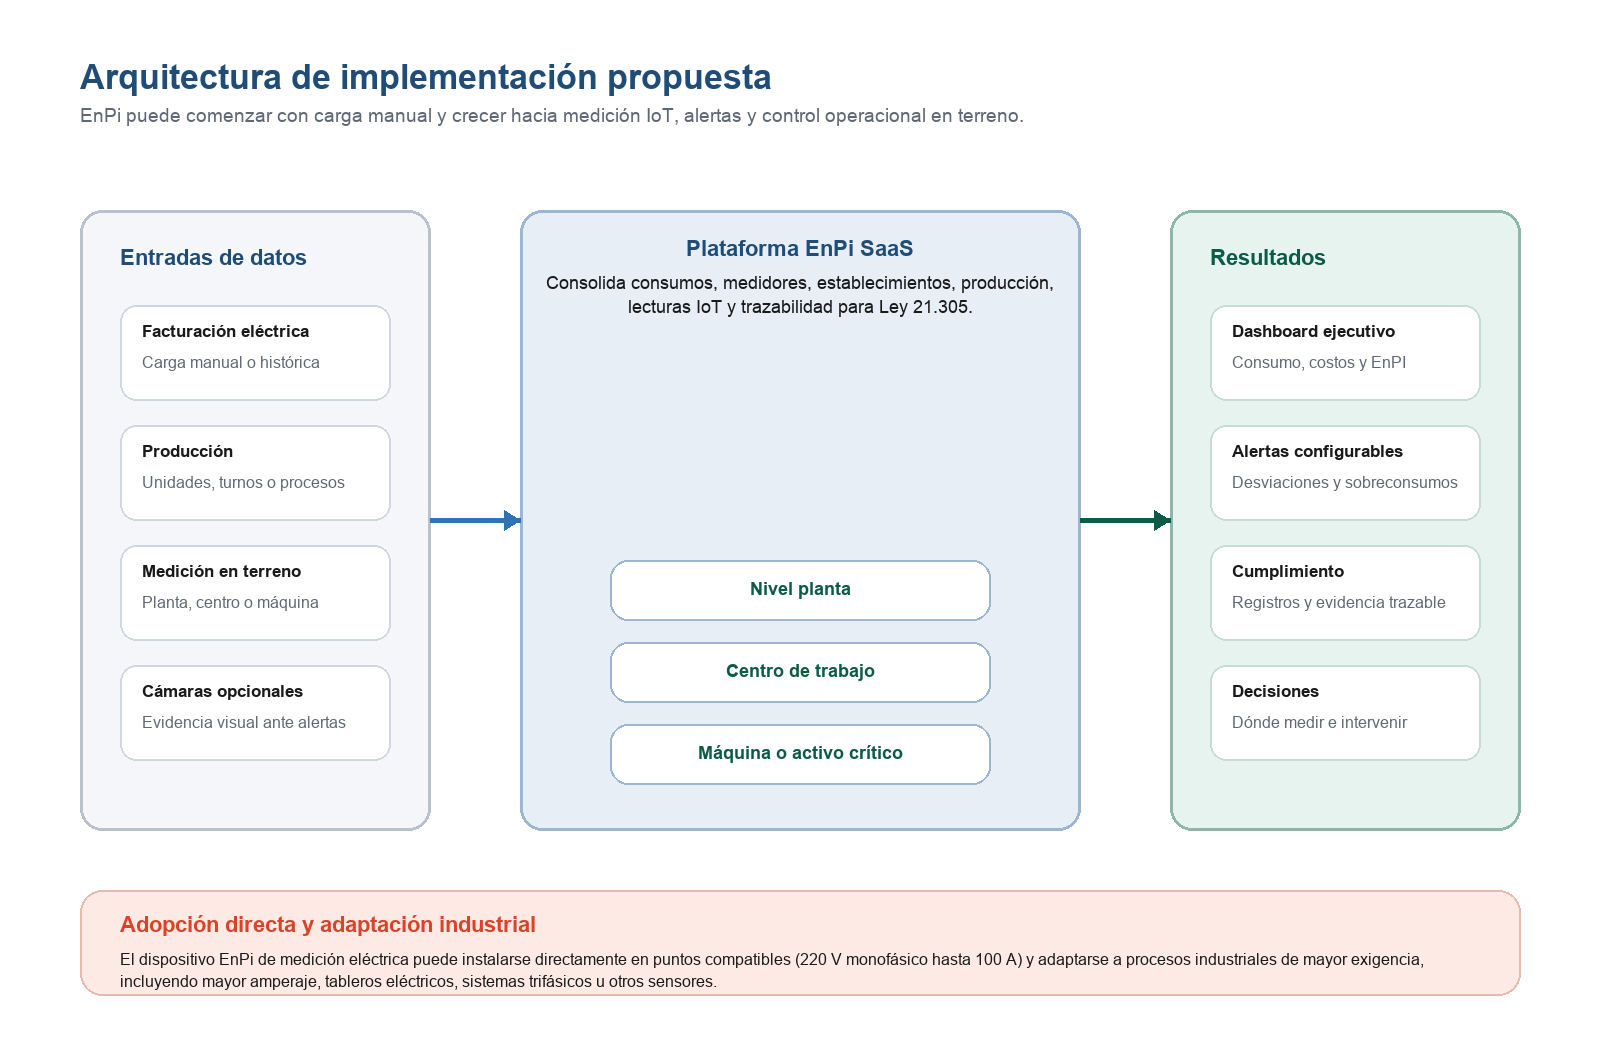
\includegraphics[width=0.92\textwidth]{figures/image1.png}
\caption{Conceptual EnPi implementation architecture: integration of manual inputs, IoT metering, SaaS platform, and outputs for energy management.}
\label{fig:1}
\end{figure*}

\begin{table*}[t]
\caption{Functional layers of the EnPi architecture.}
\label{tab:capas-funcionales-de-la-arquitectura-enpi}
\centering
\scriptsize
\begin{adjustbox}{max width=\textwidth}
\begin{tabular}{p{0.1\textwidth}p{0.35\textwidth}p{0.35\textwidth}}
\toprule
Layer & Function & Expected outcome \\
\midrule
Acquisition & Manual upload of bills, historical records, existing meters, and IoT nodes. & Energy data captured from available sources and new measurements. \\
Integration & Normalization by company, facility, work center, machine, meter, and period. & Common model for comparing consumption and assigning responsibility. \\
SaaS & Management of users, roles, catalogs, dashboards, reports, and assets. & Centralized web access for operation, analysis, and decision-making. \\
Analytics & EnPI indicators, baselines, trends, deviations, thresholds, and alert rules. & Actionable information on energy per unit produced, process, or period. \\
Governance & Traceability of origin, responsible party, period, capture method, privacy, and data reconciliation. & Greater confidence for internal use, audit, and reporting. \\
Decision & Prioritization of improvements, follow-up of measures, evidence, and technological scaling. & Preparation of traceable evidence and continuous improvement. \\
\bottomrule
\end{tabular}
\end{adjustbox}
\end{table*}

The fifth layer is data governance, oriented toward preserving traceability, origin, date, responsible party, capture method, and reconciliation among sources. Finally, the sixth layer corresponds to business decision-making, where information is used to prioritize improvements, justify consumption, support reports, evaluate energy-efficiency actions, and prepare traceable evidence for audits or regulatory requirements, without implying automatic compliance certification.

The information flow begins with the capture of energy and production data from heterogeneous sources. Each datum is recorded with origin metadata that distinguish whether it comes from a manual entry, a bill, an existing meter, or an IoT node. The platform then associates consumption with specific operational units and relates it to production records in compatible periods. This association transforms isolated electrical data into energy performance indicators such as kWh per unit produced, kWh per batch, kWh per shift, or kWh per machine.

In the IoT deployment, each EnPi node can be installed at a selected plant point without requiring the whole facility to be instrumented simultaneously. This strategy makes it possible to prioritize high-consumption equipment, critical machines, processes with high variability, or points with energy uncertainty.

\begin{figure*}[t]
\centering
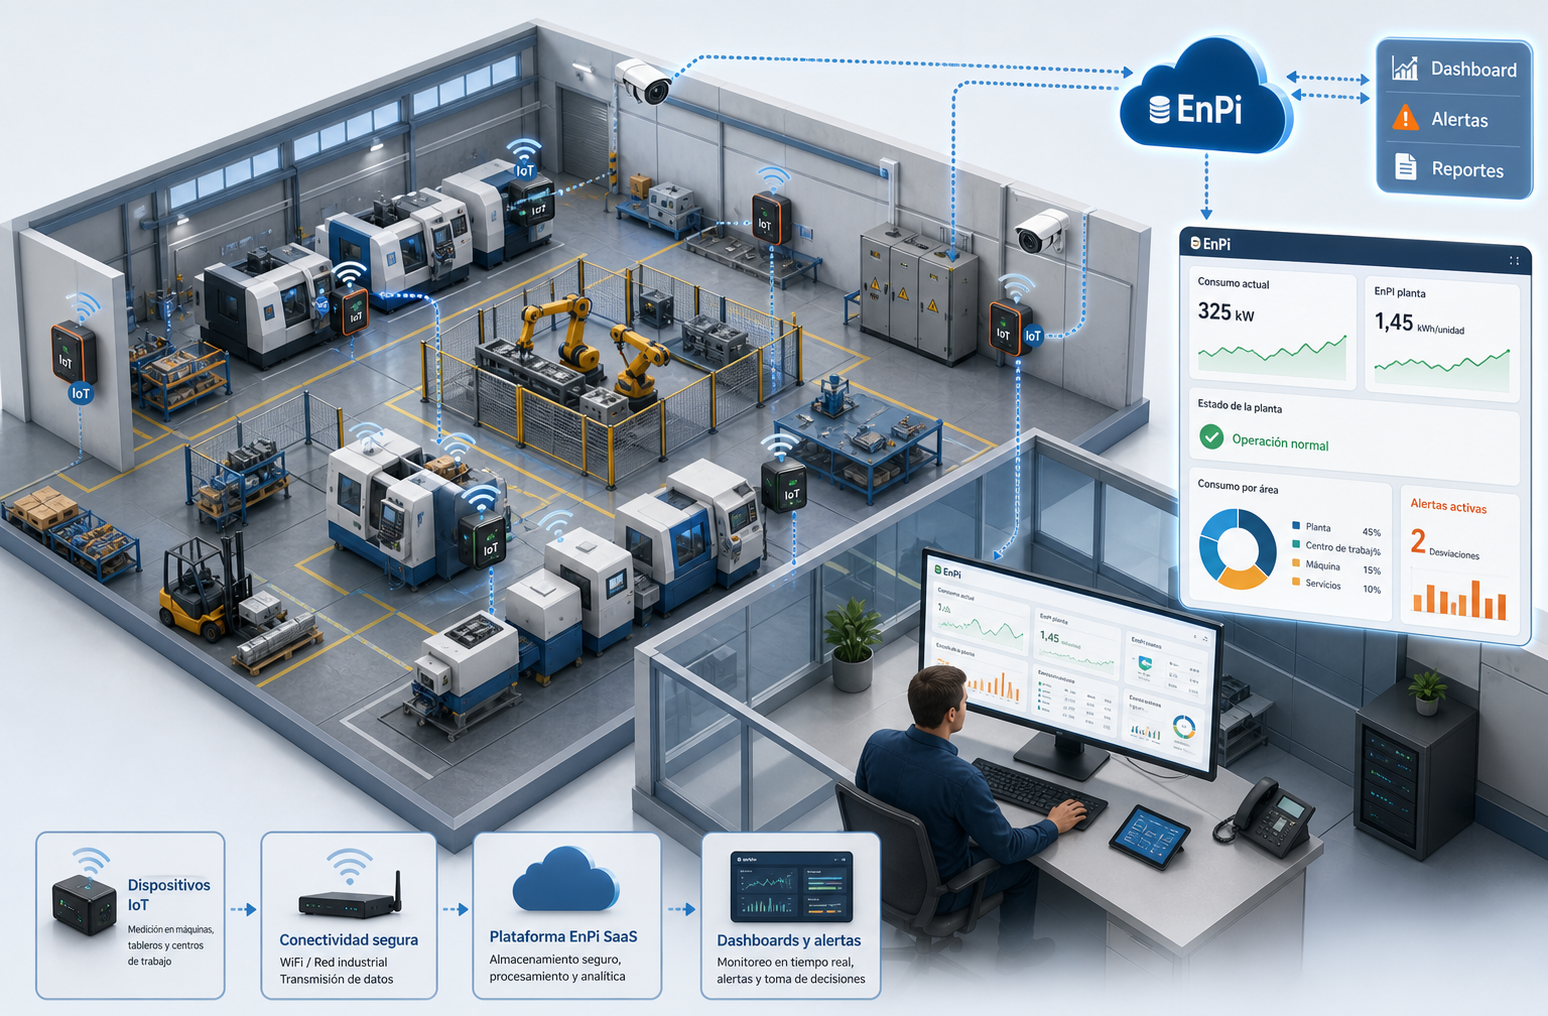
\includegraphics[width=0.92\textwidth]{figures/image2.png}
\caption{Conceptual progressive deployment scenario through intelligent energy-metering nodes and contextual support cameras for alerts.}
\label{fig:2}
\end{figure*}

Distributed metering provides temporal and spatial granularity, while the SaaS platform preserves traceability and consolidates information with manual and production data. Consequently, the architecture supports gradual adoption from basic energy records toward distributed monitoring at selected points. In the evaluated version, this statement is limited to single-phase nodes and should not be interpreted as validation of a complete industrial plant.

The architecture also allows an evolution from passive monitoring toward event-based operational responses. Alert rules can be configured on consumption thresholds, deviations from target references, after-hours operation, data loss, or abnormal variations. When an operation-defined condition is detected, the system could activate notification mechanisms or integrated contextual devices, such as cameras, alarms, or relays, provided that such devices are connected through compatible interfaces. In this manuscript, these devices are treated as architectural extensions rather than empirically validated components.

\section{EnPI Indicator and Data Model}
\label{sec:enpi-data-model}

The analytical core of EnPi is the calculation of energy performance indicators, or EnPIs, defined as metrics that relate energy consumption to a relevant operational variable. Unlike monitoring based only on absolute kWh, an EnPI allows energy consumption to be interpreted as a function of production output, operating period, or organizational unit. This distinction is important because an increase or decrease in energy use does not necessarily imply a deterioration or improvement in energy performance unless production level, shift, process, or operational context is considered at the same time.

In its basic form, the indicator is calculated as the ratio between energy consumed and production obtained during the same analysis period:

\begin{equation}
\mathrm{EnPI}=\frac{\mathrm{Energy\ consumption\ (kWh)}}{\mathrm{Production}}
\label{eq:enpi}
\end{equation}

Depending on the production process, production may be expressed as manufactured units, batches, tons, square meters, operating hours, delivered services, or another physical or economic variable defined by the company.

\begin{figure*}[!t]
\centering
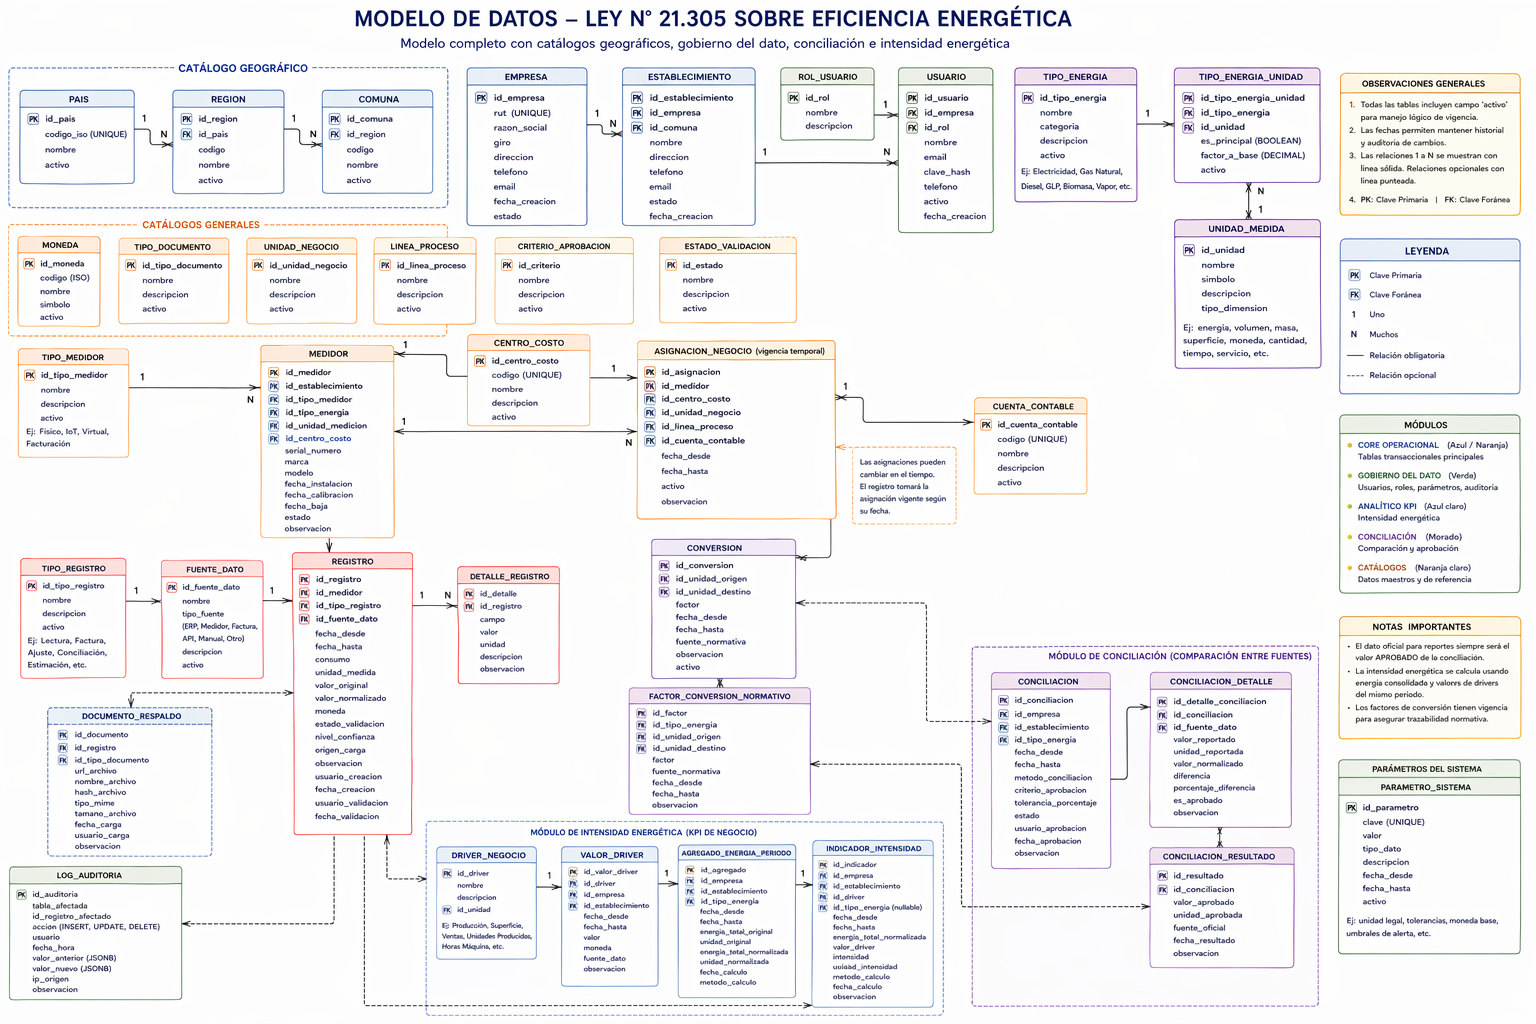
\includegraphics[width=0.92\textwidth]{figures/image3.png}
\caption{Conceptual EnPi data model for energy traceability, production, reconciliation, and energy performance indicators.}
\label{fig:data-model}
\end{figure*}

The usefulness of the indicator critically depends on data traceability. For an EnPI to be interpretable, it is not enough to store a consumption value and a production value; both must be associated with a compatible period, a capture source, an operational unit, and a responsible party or registration mechanism. EnPi addresses this requirement through a relational data model that links company, facility, meter, equipment, consumption, production, data source, target reference, reconciliation, and audit entities. This structure preserves the origin of each record, distinguishes manual from IoT data, and maintains evidence on how the information was generated.

The data model organizes information into three main groups. The first group includes organizational and physical entities such as company, facility, work center, machine, meter, and IoT node. The second group includes transactional entities where consumption records, IoT readings, production records, analysis periods, and data sources are stored. The third group includes analytical and governance entities, such as EnPI references, comparison rules, deviation states, source reconciliation, audit, and system parameters.

\begin{figure*}[t]
\centering
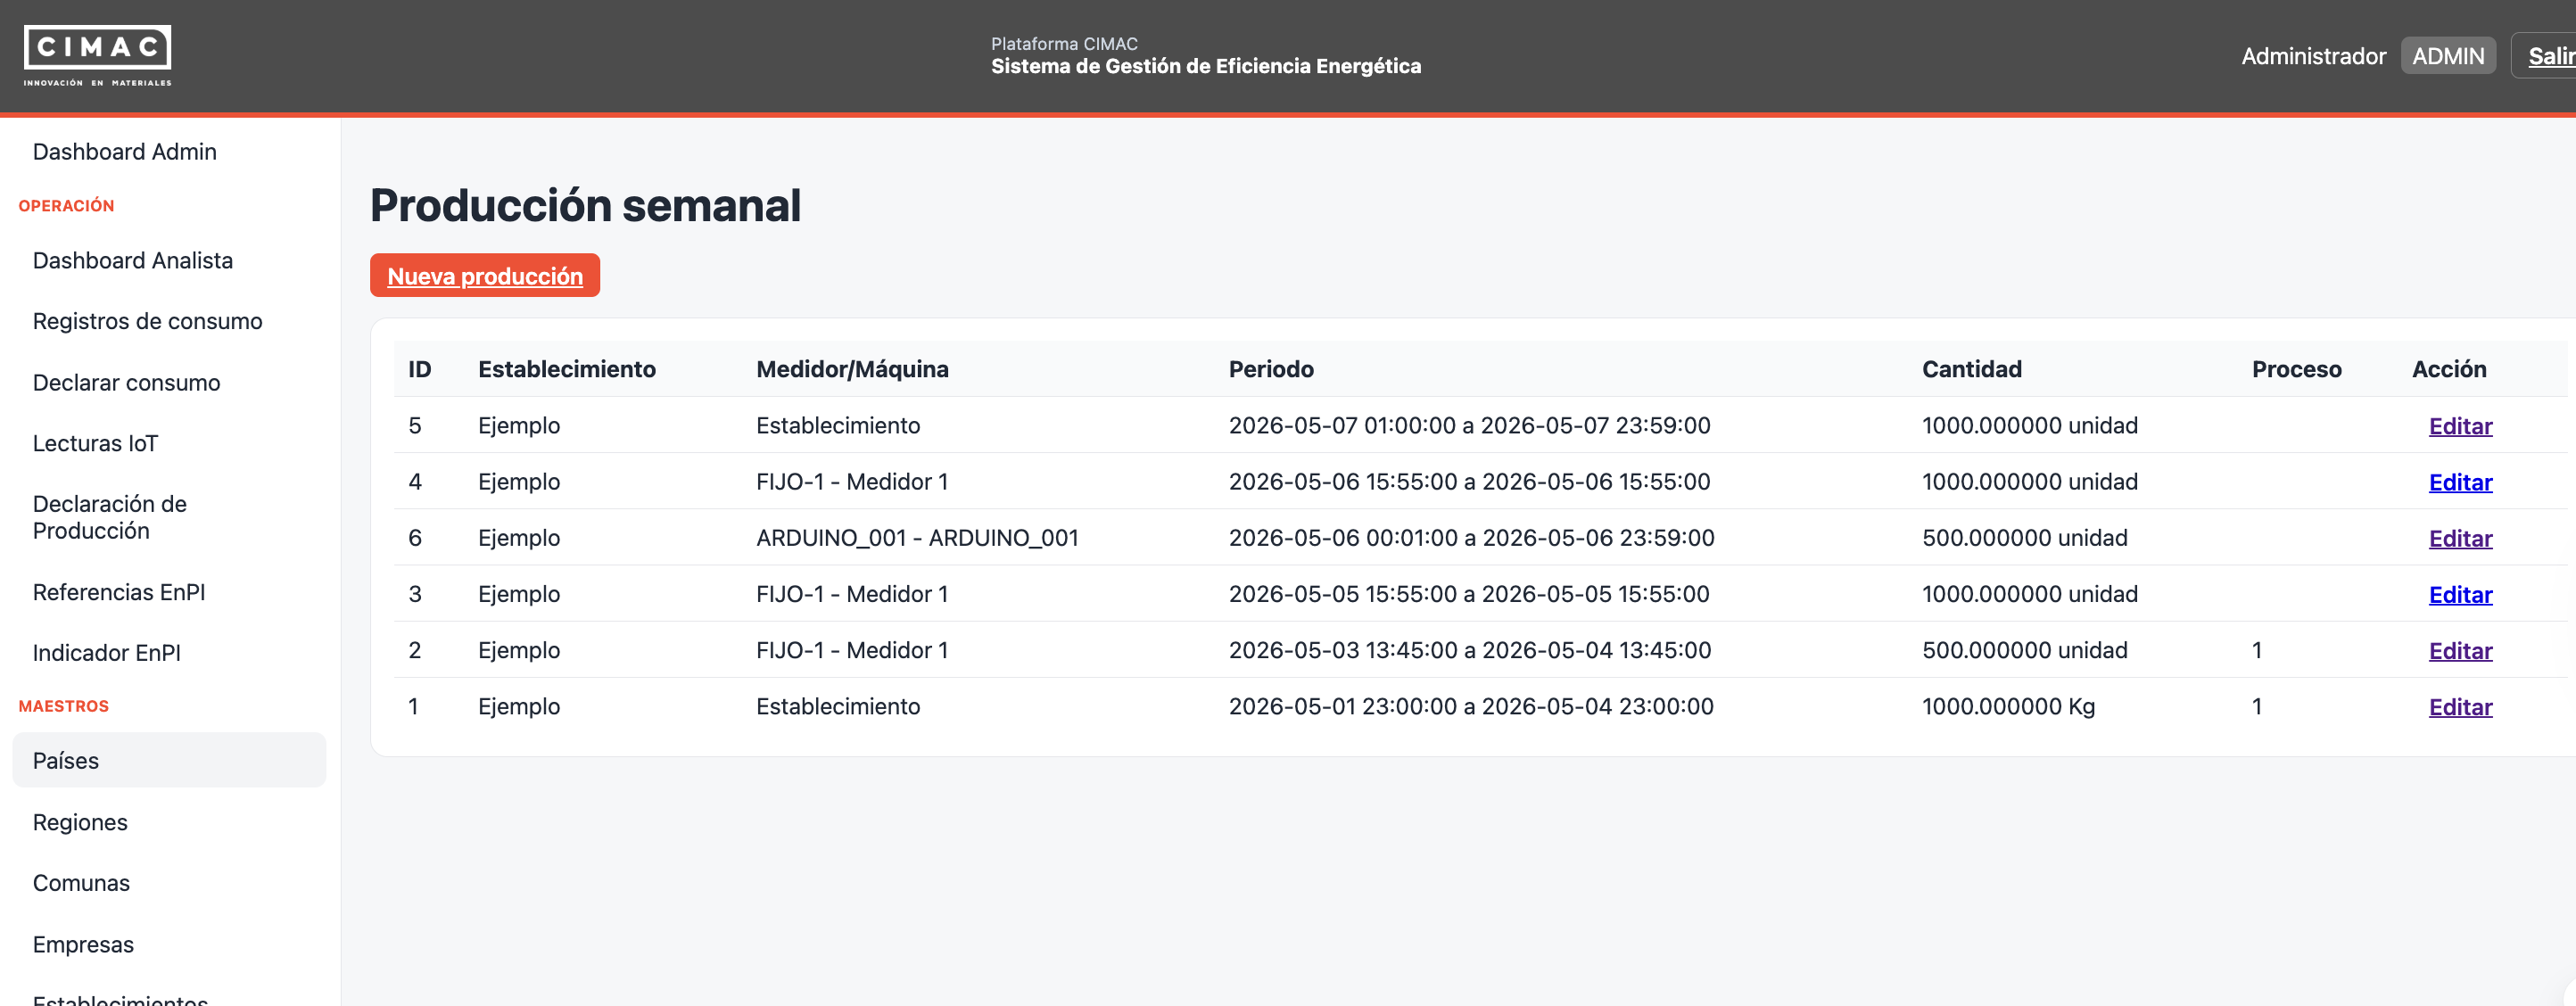
\includegraphics[width=0.92\textwidth]{figures/image4.png}
\caption{Weekly production module used to relate consumed energy to production quantity by facility, machine, or period.}
\label{fig:4}
\end{figure*}

\subsection{Anonymized Real EnPI Traceability Case}
\label{subsec:real-enpi-case}

To make explicit the traceability chain that the architecture seeks to preserve, a preliminary real case in an anonymized food-sector SME was incorporated. The metering point corresponded to a single-phase dough sheeter used to process dough. The company reported a production of 44 kg of dough per production day, and the EnPi node recorded IoT readings for 17 consecutive production days between July 31 and August 16, 2026. Due to a conversion problem observed in some processed columns, the electrical variables used for the case were reconstructed from the \texttt{payload\_raw} field, where the original values reported by the device were preserved.

Daily consumption was estimated from positive increments of the corrected energy counter, and the EnPI was calculated as kWh per kg of processed dough. As an initial operational reference, the platform used 0.0228 kWh/kg. This reference should not be interpreted as an official standard or certified target; its role is to illustrate how EnPi compares observed performance against an operational baseline. Previous studies in bakeries have reported specific ranges for kneading and related processes that vary widely according to product, scale, equipment, and operation [22], [23].

The 17-day period accumulated 17.987 kWh for a declared production of 748 kg, resulting in a weighted EnPI of 0.0240 kWh/kg and a median daily EnPI of 0.0222 kWh/kg. The alert logic classified 12 days as green, one day as warning, and four days as critical. Critical days were observed on August 4, August 7, August 10, and August 14, 2026, with deviations between +33.67\% and +59.99\% relative to the operational reference. 

\begin{table}[H]
\caption{Summary of the anonymized 17-day EnPI operational case in a food-sector SME dough sheeter.}
\label{tab:caso-real-summary}
\centering
\scriptsize
\begin{tabular}{p{0.55\columnwidth}p{0.35\columnwidth}}
\toprule
Metric & Value \\
\midrule
Operational period & 2026-07-31 to 2026-08-16 \\
Production days & 17 \\
Declared production & 44 kg/day \\
Total production & 748 kg \\
Total measured energy & 17.987 kWh \\
Weighted EnPI & 0.0240 kWh/kg \\
Median daily EnPI & 0.0222 kWh/kg \\
Operational reference & 0.0228 kWh/kg \\
Minimum daily EnPI & 0.0173 kWh/kg \\
Maximum daily EnPI & 0.0365 kWh/kg \\
Status distribution & 12 green, 1 warning, 4 critical \\
\bottomrule
\end{tabular}
\end{table}

These deviations allowed the business owner to review possible operational causes of abnormal energy intensity, such as differences in the number of dough passes, idle operation, cleaning periods, scheduling, or effective machine loading. The platform did not infer those causes automatically; rather, it provided traceable evidence to prioritize and structure the operational diagnosis. 

The case shows that the minimum chain required by EnPi can be reconstructed from raw data to operational decision: IoT reading in \texttt{payload\_raw}, correction of physical variables, daily energy estimation, association with the operational object, reconciliation with daily production, EnPI calculation, comparison against a reference, dashboard visualization, and status registration. This sequence allows the indicator to be traced from the final value back to the sources that originated it.


\begin{table}[H]
\caption{Critical days identified by the EnPi alert logic during the operational use case.}
\label{tab:critical-days}
\centering
\scriptsize
\begin{tabular}{p{0.28\columnwidth}p{0.24\columnwidth}p{0.22\columnwidth}p{0.16\columnwidth}}
\toprule
Date & EnPI & Deviation & Status \\
\midrule
2026-08-04 & 0.0339 kWh/kg & +48.82\% & Critical \\
2026-08-07 & 0.0365 kWh/kg & +59.99\% & Critical \\
2026-08-10 & 0.0337 kWh/kg & +47.73\% & Critical \\
2026-08-14 & 0.0305 kWh/kg & +33.67\% & Critical \\
\bottomrule
\end{tabular}
\end{table}

\begin{figure*}[!t]
\centering
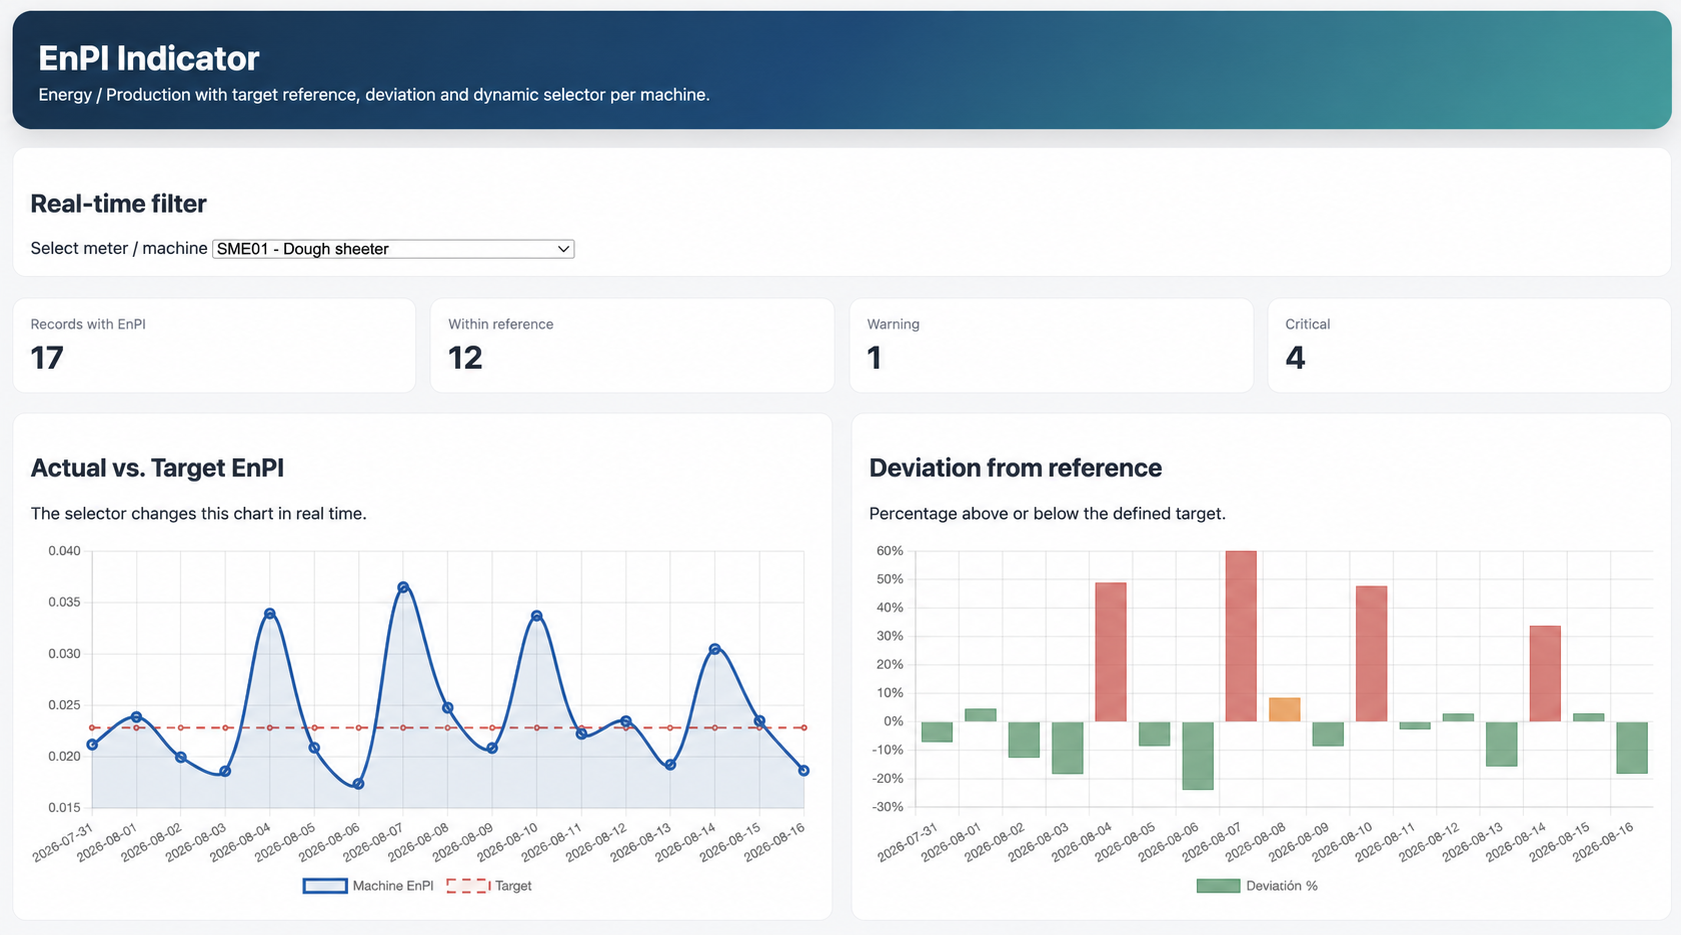
\includegraphics[width=0.92\textwidth]{figures/enpi_dashboard_sme01_dough_sheeter.png}
\caption{Operational EnPI dashboard for the anonymized food-sector SME use case. The platform summarizes 17 daily EnPI records for the monitored dough sheeter, including 12 days within reference, one warning day, and four critical days. The left panel compares daily EnPI against the operational target, while the right panel shows percentage deviation from the reference.}
\label{fig:enpi-dashboard-sme}
\end{figure*}

\begin{table*}[!t]
\caption{Daily EnPI records for the anonymized food-sector SME dough sheeter. Declared production was 44 kg of dough per production day; the operational reference was 0.0228 kWh/kg.}
\label{tab:caso-real-enpi}
\centering
\scriptsize
\begin{adjustbox}{max width=\textwidth}
\begin{tabular}{p{0.12\textwidth}p{0.11\textwidth}p{0.12\textwidth}p{0.12\textwidth}p{0.12\textwidth}p{0.12\textwidth}p{0.11\textwidth}p{0.12\textwidth}}
\toprule
Date & Energy & Production & Observed EnPI & Reference & Deviation & Status & Traceability chain \\
\midrule
2026-07-31 & 0.932 kWh & 44 kg & 0.0212 kWh/kg & 0.0228 kWh/kg & -7.10\% & Green & \texttt{payload\_raw} $\rightarrow$ kWh $\rightarrow$ kg $\rightarrow$ EnPI $\rightarrow$ status \\
2026-08-01 & 1.049 kWh & 44 kg & 0.0238 kWh/kg & 0.0228 kWh/kg & +4.57\% & Green & \texttt{payload\_raw} $\rightarrow$ kWh $\rightarrow$ kg $\rightarrow$ EnPI $\rightarrow$ status \\
2026-08-02 & 0.876 kWh & 44 kg & 0.0199 kWh/kg & 0.0228 kWh/kg & -12.68\% & Green & \texttt{payload\_raw} $\rightarrow$ kWh $\rightarrow$ kg $\rightarrow$ EnPI $\rightarrow$ status \\
2026-08-03 & 0.818 kWh & 44 kg & 0.0186 kWh/kg & 0.0228 kWh/kg & -18.46\% & Green & \texttt{payload\_raw} $\rightarrow$ kWh $\rightarrow$ kg $\rightarrow$ EnPI $\rightarrow$ status \\
2026-08-04 & 1.493 kWh & 44 kg & 0.0339 kWh/kg & 0.0228 kWh/kg & +48.82\% & Critical & \texttt{payload\_raw} $\rightarrow$ kWh $\rightarrow$ kg $\rightarrow$ EnPI $\rightarrow$ status \\
2026-08-05 & 0.917 kWh & 44 kg & 0.0208 kWh/kg & 0.0228 kWh/kg & -8.59\% & Green & \texttt{payload\_raw} $\rightarrow$ kWh $\rightarrow$ kg $\rightarrow$ EnPI $\rightarrow$ status \\
2026-08-06 & 0.763 kWh & 44 kg & 0.0173 kWh/kg & 0.0228 kWh/kg & -23.94\% & Green & \texttt{payload\_raw} $\rightarrow$ kWh $\rightarrow$ kg $\rightarrow$ EnPI $\rightarrow$ status \\
2026-08-07 & 1.605 kWh & 44 kg & 0.0365 kWh/kg & 0.0228 kWh/kg & +59.99\% & Critical & \texttt{payload\_raw} $\rightarrow$ kWh $\rightarrow$ kg $\rightarrow$ EnPI $\rightarrow$ status \\
2026-08-08 & 1.088 kWh & 44 kg & 0.0247 kWh/kg & 0.0228 kWh/kg & +8.45\% & Warning & \texttt{payload\_raw} $\rightarrow$ kWh $\rightarrow$ kg $\rightarrow$ EnPI $\rightarrow$ status \\
2026-08-09 & 0.916 kWh & 44 kg & 0.0208 kWh/kg & 0.0228 kWh/kg & -8.69\% & Green & \texttt{payload\_raw} $\rightarrow$ kWh $\rightarrow$ kg $\rightarrow$ EnPI $\rightarrow$ status \\
2026-08-10 & 1.482 kWh & 44 kg & 0.0337 kWh/kg & 0.0228 kWh/kg & +47.73\% & Critical & \texttt{payload\_raw} $\rightarrow$ kWh $\rightarrow$ kg $\rightarrow$ EnPI $\rightarrow$ status \\
2026-08-11 & 0.977 kWh & 44 kg & 0.0222 kWh/kg & 0.0228 kWh/kg & -2.61\% & Green & \texttt{payload\_raw} $\rightarrow$ kWh $\rightarrow$ kg $\rightarrow$ EnPI $\rightarrow$ status \\
2026-08-12 & 1.032 kWh & 44 kg & 0.0235 kWh/kg & 0.0228 kWh/kg & +2.87\% & Green & \texttt{payload\_raw} $\rightarrow$ kWh $\rightarrow$ kg $\rightarrow$ EnPI $\rightarrow$ status \\
2026-08-13 & 0.845 kWh & 44 kg & 0.0192 kWh/kg & 0.0228 kWh/kg & -15.77\% & Green & \texttt{payload\_raw} $\rightarrow$ kWh $\rightarrow$ kg $\rightarrow$ EnPI $\rightarrow$ status \\
2026-08-14 & 1.341 kWh & 44 kg & 0.0305 kWh/kg & 0.0228 kWh/kg & +33.67\% & Critical & \texttt{payload\_raw} $\rightarrow$ kWh $\rightarrow$ kg $\rightarrow$ EnPI $\rightarrow$ status \\
2026-08-15 & 1.033 kWh & 44 kg & 0.0235 kWh/kg & 0.0228 kWh/kg & +2.97\% & Green & \texttt{payload\_raw} $\rightarrow$ kWh $\rightarrow$ kg $\rightarrow$ EnPI $\rightarrow$ status \\
2026-08-16 & 0.820 kWh & 44 kg & 0.0186 kWh/kg & 0.0228 kWh/kg & -18.26\% & Green & \texttt{payload\_raw} $\rightarrow$ kWh $\rightarrow$ kg $\rightarrow$ EnPI $\rightarrow$ status \\
\bottomrule
\end{tabular}
\end{adjustbox}
\end{table*}



\section{Functional Implementation of the SaaS Platform}
\label{sec:functional-implementation}

The functional implementation of EnPi materializes the proposed architecture in a SaaS platform oriented toward the operational management of energy and production information. The platform manages users, companies, facilities, meters, machines or metering points, consumption records, IoT readings, production, target references, and EnPI indicators. This implementation transforms the conceptual model into a traceable workflow: manual and IoT sources feed the energy database, production records provide the operational denominator, and the analytical module calculates energy performance against organization-defined references.

Operationally, the platform was designed so that a company can begin with available information and gradually increase the level of digitalization. In an initial stage, users can enter historical consumption, electricity bills, existing meters, and production by period. In later stages, the company can incorporate IoT nodes associated with machines, work centers, or specific panels. This logic allows the system to combine manual records, historical data, and distributed metering within the same traceability structure.

Figure~\ref{fig:4} shows the production module, where users register produced quantities associated with a facility, machine, period, or operational unit. This component is central because it converts energy consumption into an energy-intensity indicator. Without a compatible production record, the platform could only report absolute kWh; with associated production, EnPi can calculate indicators such as kWh per unit, kWh per batch, kWh per shift, or kWh per work center.

This functionality converts energy and production records into an actionable metric for prioritizing critical equipment, reviewing processes, configuring alerts, or evaluating energy-efficiency measures. The operational case dashboard in Figure~\ref{fig:enpi-dashboard-sme} illustrates this analytical layer with real anonymized records, showing the daily EnPI, the reference value, and the resulting alert status. Complementarily, Figure~\ref{fig:6} shows the platform dashboard used to inspect consumption records, raw IoT readings, and validation or linking states. This component makes it possible to review the raw information that feeds the indicators, verify whether a reading comes from an IoT node or manual entry, and preserve evidence about the origin of each datum.

\begin{figure*}[t]
\centering
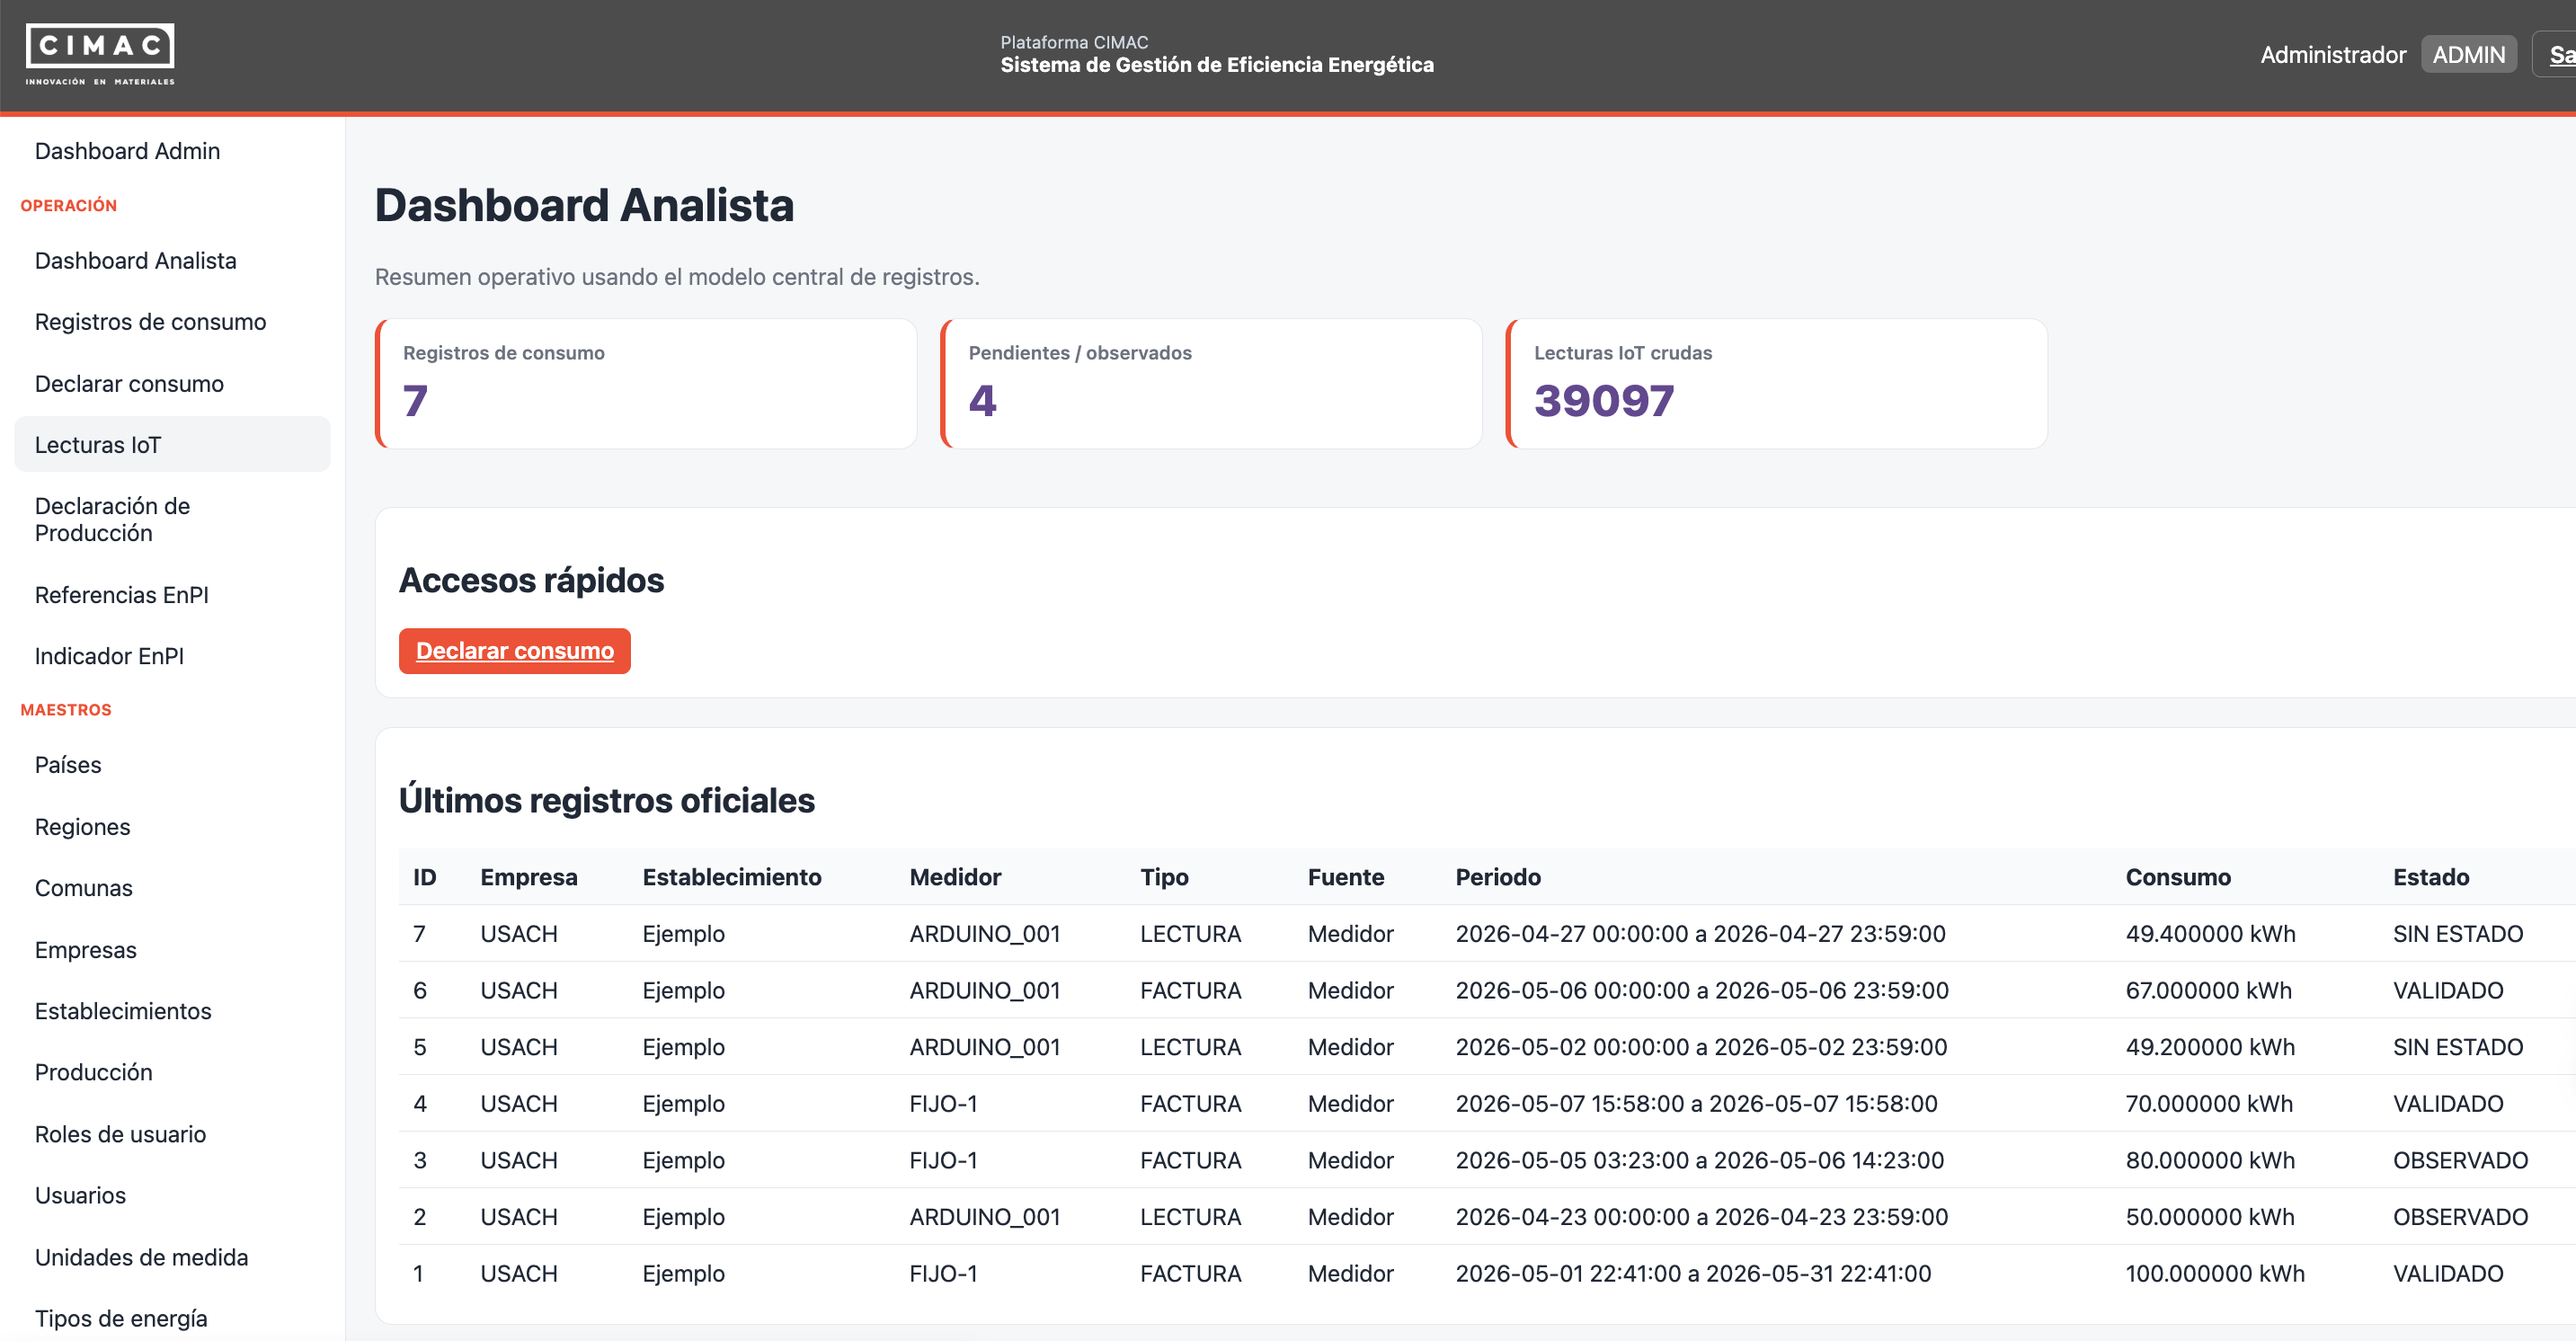
\includegraphics[width=\textwidth]{figures/image6.png}
\caption{Operational dashboard with consumption records, raw IoT readings, and energy-data validation status.}
\label{fig:6}
\end{figure*}

\section{Progressive Adoption Model}
\label{sec:progressive-adoption}

A central contribution of EnPi is organizing technology adoption into incremental levels so that companies do not need to implement complete plant instrumentation from the start. At the first level, an organization can upload electricity bills, historical records, and manual operational data to build an initial energy baseline. At the second level, consumption can be associated with facilities, work centers, machines, or relevant assets. At the third level, IoT nodes are incorporated at critical points where granular metering adds economic or operational value. Subsequent levels may extend the platform toward three-phase metering, electrical panels, alert rules, contextual devices, operational-support cameras, and advanced analytics.

This approach reduces entry barriers by prioritizing metering points with higher uncertainty, consumption, or production criticality. Instead of requiring a large initial investment, EnPi allows selective node deployment and gradual coverage expansion according to budget availability, connectivity, digital maturity, and expected information return. Methodologically, the model proposes a transition between energy management based on ex post records and management based on energy performance indicators calculated from continuous operational evidence.

\begin{figure}[H]
\centering
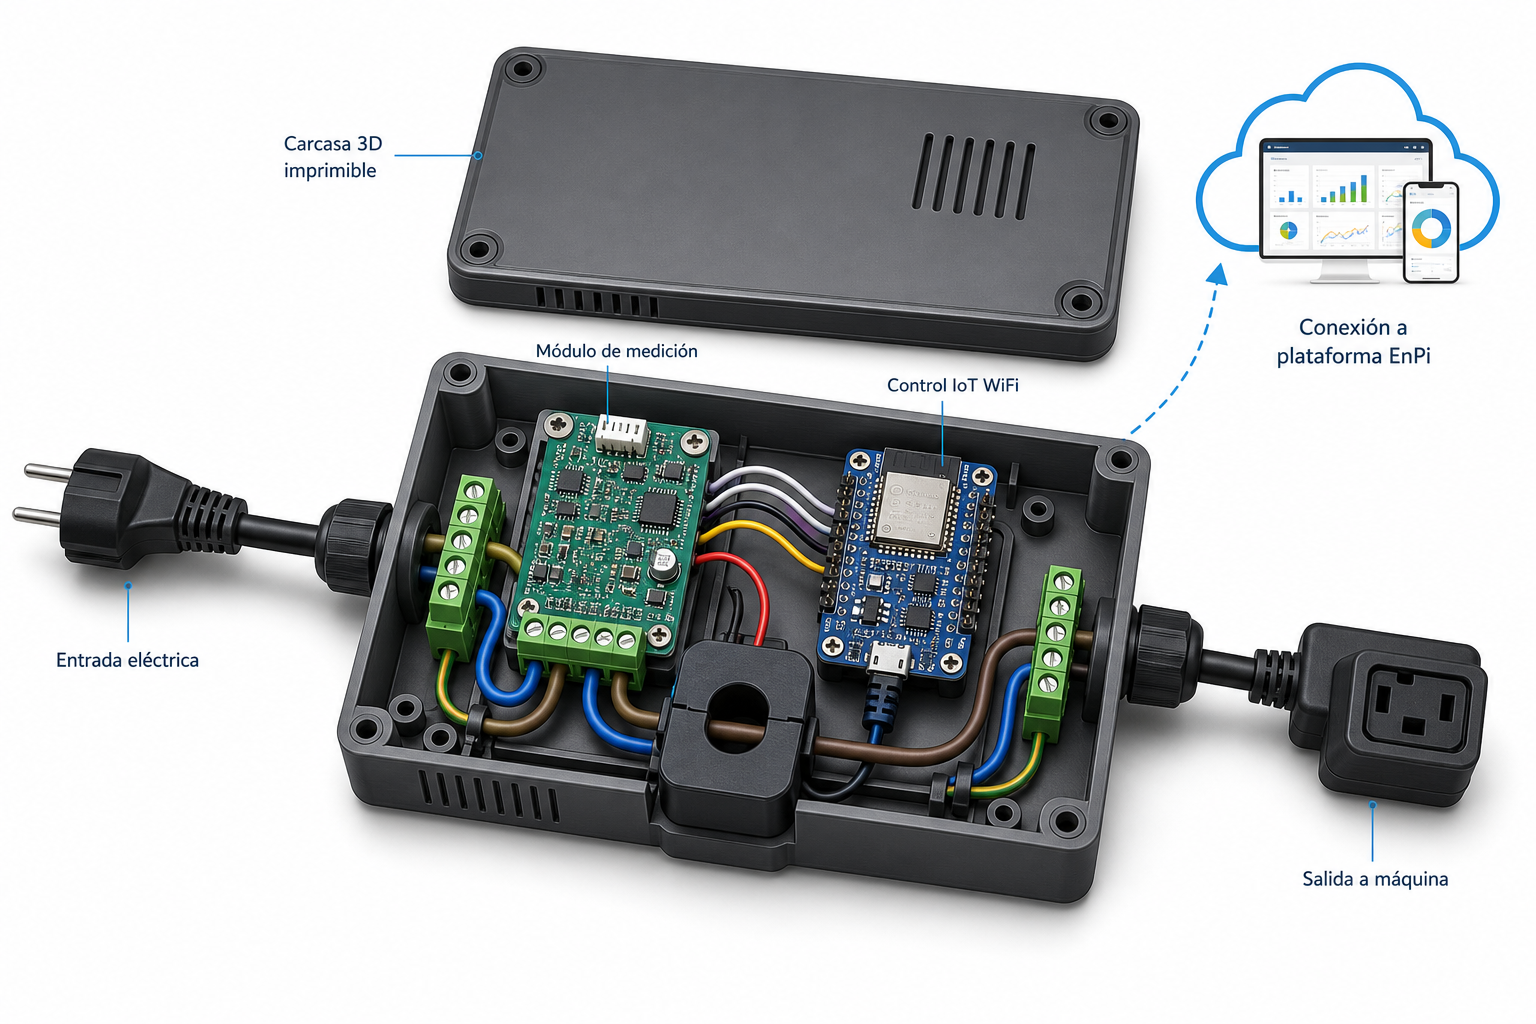
\includegraphics[width=\columnwidth]{figures/image7.png}
\caption{Representation of the single-phase plug-and-play node used as an IoT metering artifact in the preliminary experimental campaign.}
\label{fig:7}
\end{figure}

To support progressive adoption, the EnPi plug-and-play node includes an assisted installation procedure intended to reduce dependence on specialized personnel. Each device is delivered with a physical installation sheet that includes summarized instructions, local access credentials, and a QR code to register the company, facility, and module or meter in the web platform. This mechanism links the physical deployment of the device with its digital record, preventing the installation from becoming disconnected from asset traceability within the EnPi ecosystem.

\begin{figure}[H]
\centering
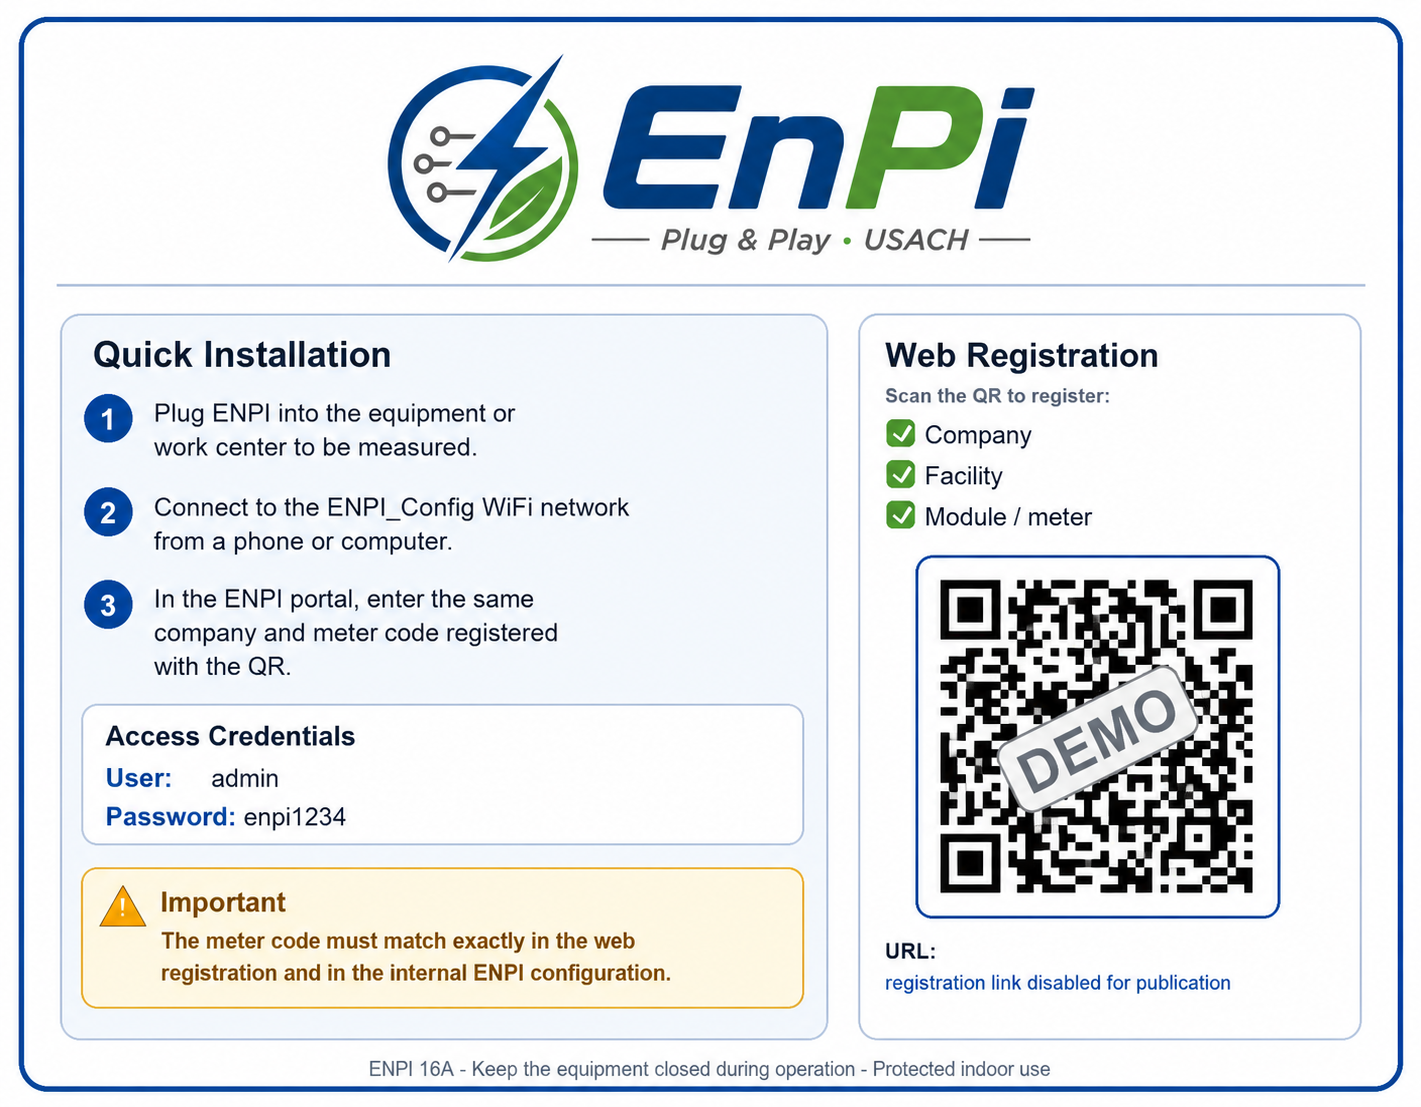
\includegraphics[width=\columnwidth]{adhesivo_enpi.png}
\caption{Physical installation sheet for the EnPi plug-and-play node, used to link the device with the web record, company, facility, and meter code before automatic measurement begins.}
\label{fig:ficha-instalacion-enpi}
\end{figure}

Each metering point is associated with a company, facility, meter, operational location, and data source. This increases energy-monitoring granularity while maintaining consistent traceability between the physical device, the IoT reading, and the EnPI indicator calculated by the platform. Consequently, progressive adoption is not only a technology-growth strategy but also an operational procedure for deploying, registering, and maintaining distributed metering nodes in the field.

\section{Experimental Methodology}
\label{sec:experimental-methodology}
The experimental validation was carried out through parallel measurement between a single-phase plug-and-play EnPi node and a Metrel MI2883 power quality analyzer with valid calibration. The available calibration certificate corresponds to CCE:814-2025, dated 20-10-2025. The objective was to evaluate the agreement between measurements obtained by EnPi and a reference instrument under different electrical-load scenarios representative of operational use.

The test considered 10 single-phase load scenarios, including no-load condition, resistive load, electronic load, inductive load, and scenarios with periodic on/off variations. In each scenario, both instruments simultaneously measured the same load circuit, keeping the EnPi current sensor and the Metrel clamps on the same phase conductor. Measurements were then temporally paired by timestamp rounded to the second to compare the series obtained by both systems.

\begin{table}[H]
\caption{Real EnPi-Metrel validation scenarios and paired samples.}
\label{tab:escenarios-reales-de-validacion-de-enpi-metre}
\centering
\begin{adjustbox}{max width=\columnwidth}
\begin{tabular}{p{0.1\textwidth}p{0.35\textwidth}p{0.1\textwidth}}
\toprule
Scenario & Description & Samples \\
\midrule
000 & No load (test 1) & 577 \\
001 & Light bulb & 1202 \\
002 & Laptop charging & 1191 \\
003 & Heater & 900 \\
004 & Mobile phone charging & 1201 \\
005 & Angle grinder & 1201 \\
006 & Monitor & 1201 \\
007 & Mixed: heater + mobile phone + laptop + light bulb & 1181 \\
008 & No load (test 2) & 900 \\
009 & Heater with power variations & 1042 \\
\bottomrule
\end{tabular}
\end{adjustbox}
\end{table}

The EnPi node recorded voltage, current, active power, accumulated energy, frequency, and power factor, transmitting the readings to the SaaS-IoT platform with timestamp, meter code, and origin traceability. The metering hardware was based on a PZEM-004T TTL Modbus-RTU single-phase 100 A module integrated into the firmware through the \texttt{PZEM004Tv30} library. According to the commercial data sheet used for acquisition, this variant operates nominally at 80--260 VAC, 0--100 A, 45--65 Hz, and power factor 0--1. The module was installed inside a plug-and-play adapter: the live conductor feeding the dough sheeter passes through the internal metering point, and internal terminal blocks connect male and female plugs to interpose the node between the grid and the machine without modifying the fixed installation. Transmission was performed by an ESP32S3 with firmware 1.0, configured with a 60,000 ms reading interval, NTP time synchronization, and direct HTTPS delivery to the server. The \texttt{payload\_raw} field corresponds to the raw reading transmitted from the ESP32S3, without intermediate backend transformation before storage.

\section{Preliminary Experimental Validation Against Metrel MI2883}
\label{sec:metrel-validation}

This section presents the preliminary experimental validation of the EnPi node through direct comparison with a calibrated Metrel MI2883 power quality analyzer, certificate CCE:814-2025 and calibration date 20-10-2025. Metrel was used as the operational reference instrument at this stage, while EnPi was evaluated as an IoT node for operational energy monitoring in controlled single-phase scenarios. This validation should not be interpreted as a complete industrial test of the SaaS-IoT platform or as metrological certification of the device.

The study uses 10 load scenarios and 10,596 paired samples. Records were aligned by scenario and timestamp rounded to the second, preserving continuous segments and excluding unpaired records before error calculation. The control sheet documents 163 unpaired records, equivalent to approximately 1.51\% of the total observed. These cases corresponded to packet losses toward the server and are reported as part of IoT continuity, not as metrological error. After this behavior was identified, the firmware was modified to temporarily store non-transmitted readings and re-inject them when the connection became available; this improvement is outside the already compared dataset.

\subsection{Metrics and Comparison Criteria}
\label{subsec:metrics-criteria}

MAE, RMSE, MAPE, WMAPE, mean bias, Pearson correlation, R\textasciicircum{}2, and Bland-Altman limits of agreement were calculated. MAE interprets error in physical units; RMSE penalizes larger deviations; MAPE facilitates relative comparison between loaded scenarios; and Bland-Altman analysis identifies systematic bias between instruments. In no-load scenarios, current and power-factor MAPE are not reported because the denominator tends toward zero and the metric loses physical interpretation. To avoid excessive metrological interpretation, we contrasted results against operational acceptability criteria rather than certification classes. These criteria are supported by three contextual references: the typical specification of low-cost PZEM modules, IoT studies validating PZEM-based monitors against commercial devices, and IEC energy-meter error limits as a reference framework, without claiming certification or regulatory conformity [24], [25].

\begin{table*}[t]
\caption{Reproducibility information for the EnPi node and experimental pairing.}
\label{tab:reproducibilidad-minima}
\centering
\scriptsize
\begin{adjustbox}{max width=\textwidth}
\begin{tabular}{p{0.20\textwidth}p{0.36\textwidth}p{0.36\textwidth}}
\toprule
Element & Status in this version & Requirement before final submission \\
\midrule
Node hardware & ESP32S3 as transmission unit and PZEM-004T TTL Modbus-RTU single-phase 100 A module, integrated through \texttt{PZEM004Tv30}. Nominal range according to the commercial data sheet: 80--260 VAC, 0--100 A, 45--65 Hz, and power factor 0--1. The module was housed in a plug-and-play adapter with internal terminal blocks and male/female plugs; the live conductor feeding the dough sheeter passes through the internal metering point. & Commercial or technical data sheet retained in the internal study file. \\
Firmware and sampling & Firmware 1.0; 60,000 ms reading interval; NTP time synchronization; direct HTTPS delivery to the server. After the campaign, temporary storage and re-injection of readings were incorporated for packet-loss events. & The firmware is kept internally and will not be publicly disclosed; hash or version may be documented if project policy allows it. \\
Payload and transformation & \texttt{payload\_raw} corresponds to the raw reading transmitted by the ESP32S3; no intermediate backend transformation exists before storage. & Raw payload field retained as auditable evidence; subsequent corrections are documented. \\
Temporal pairing & Alignment by scenario and timestamp rounded to the second between EnPi and Metrel; exclusion of 163 unpaired records due to packet loss toward the server, equivalent to 1.51\%. & Pairing control sheet and exclusion criterion retained in the internal audit material. \\
Metrel MI2883 & Power quality analyzer used as the operational reference, with calibration certificate CCE:814-2025 and calibration date 20-10-2025; simultaneous measurement on the same circuit/phase conductor. & Calibration certificate and export configuration retained in the internal study file. \\
Data and code & The raw data and processed data used to support the reported analysis are publicly available in the EnPi repository at \url{https://github.com/The-Terial/Enpi}. The node firmware is documented by version; if the complete firmware cannot be released, a version identifier or hash should be retained for auditability. & The final data availability statement should cite the repository and identify the folders or files that reproduce the EnPi--Metrel comparison and operational case. \\
\bottomrule
\end{tabular}
\end{adjustbox}
\end{table*}

\begin{table}[H]
\caption{Operational acceptance criteria used to interpret the EnPi--Metrel comparison. These thresholds do not constitute metrological certification.}
\label{tab:criterios-operacionales}
\centering
\scriptsize
\begin{adjustbox}{max width=\columnwidth}
\begin{tabular}{p{0.23\columnwidth}p{0.30\columnwidth}p{0.39\columnwidth}}
\toprule
Variable & Operational criterion & Justification \\
\midrule
Voltage & MAE $<$ 2 V & Suitable for operational monitoring in 220--230 V single-phase networks. \\
Current under load & MAPE $<$ 10\% and joint review with MAE & Percentage error is informative under load; at low current, absolute error should be prioritized. \\
Frequency & MAE $<$ 0.1 Hz & The grid varies little; small absolute differences can reduce correlation without operational impact. \\
Power factor & MAE $<$ 0.03 & Sufficient to classify resistive, inductive, electronic, or mixed profiles in energy management. \\
Active power & Exploratory & Calculated from Metrel variables rather than from a direct active-power column exported by the instrument. \\
\bottomrule
\end{tabular}
\end{adjustbox}
\end{table}

\begin{table*}[t]
\caption{Scenario-level error for variables directly measured against the Metrel MI2883. N/A indicates no-load scenarios or near-zero denominators, where MAPE has no robust physical interpretation and MAE should be prioritized.}
\label{tab:error-por-escenario-para-variables-medidas-di}
\centering
\scriptsize
\begin{adjustbox}{max width=\textwidth}
\begin{tabular}{cccccccccc}
\toprule
Sc. & n & MAE V & MAPE V & MAE I & MAPE I & MAE f & MAPE f & MAE PF & MAPE PF \\
\midrule
000 & 577 & 0.832 & 0.36\% & 0.0397 & N/A & 0.047 & 0.06\% & N/A & N/A \\
001 & 1202 & 0.832 & 0.36\% & 0.0110 & 3.94\% & 0.042 & 0.06\% & 0.0107 & 0.01\% \\
002 & 1191 & 0.840 & 0.37\% & 0.0112 & 3.41\% & 0.047 & 0.06\% & 0.0077 & 0.03\% \\
003 & 900 & 0.840 & 0.37\% & 0.1335 & 1.65\% & 0.071 & 0.08\% & 0.0030 & 0.00\% \\
004 & 1201 & 0.853 & 0.37\% & 0.0120 & 7.80\% & 0.071 & 0.08\% & N/A & N/A \\
005 & 1201 & 0.945 & 0.41\% & 0.0557 & 3.75\% & 0.066 & 0.07\% & 0.0017 & 0.00\% \\
006 & 1201 & 0.927 & 0.40\% & 0.0116 & 3.37\% & 0.054 & 0.06\% & 0.0126 & 0.01\% \\
007 & 1181 & 0.940 & 0.41\% & 0.1672 & 1.95\% & 0.046 & 0.06\% & 0.0006 & 0.00\% \\
008 & 900 & 1.034 & 0.45\% & 0.0432 & N/A & 0.069 & 0.08\% & N/A & N/A \\
009 & 1042 & 0.922 & 0.40\% & 0.1266 & 2.45\% & 0.052 & 0.06\% & 0.0039 & 0.01\% \\
\bottomrule
\end{tabular}
\end{adjustbox}
\end{table*}

\begin{figure*}[!t]
\centering
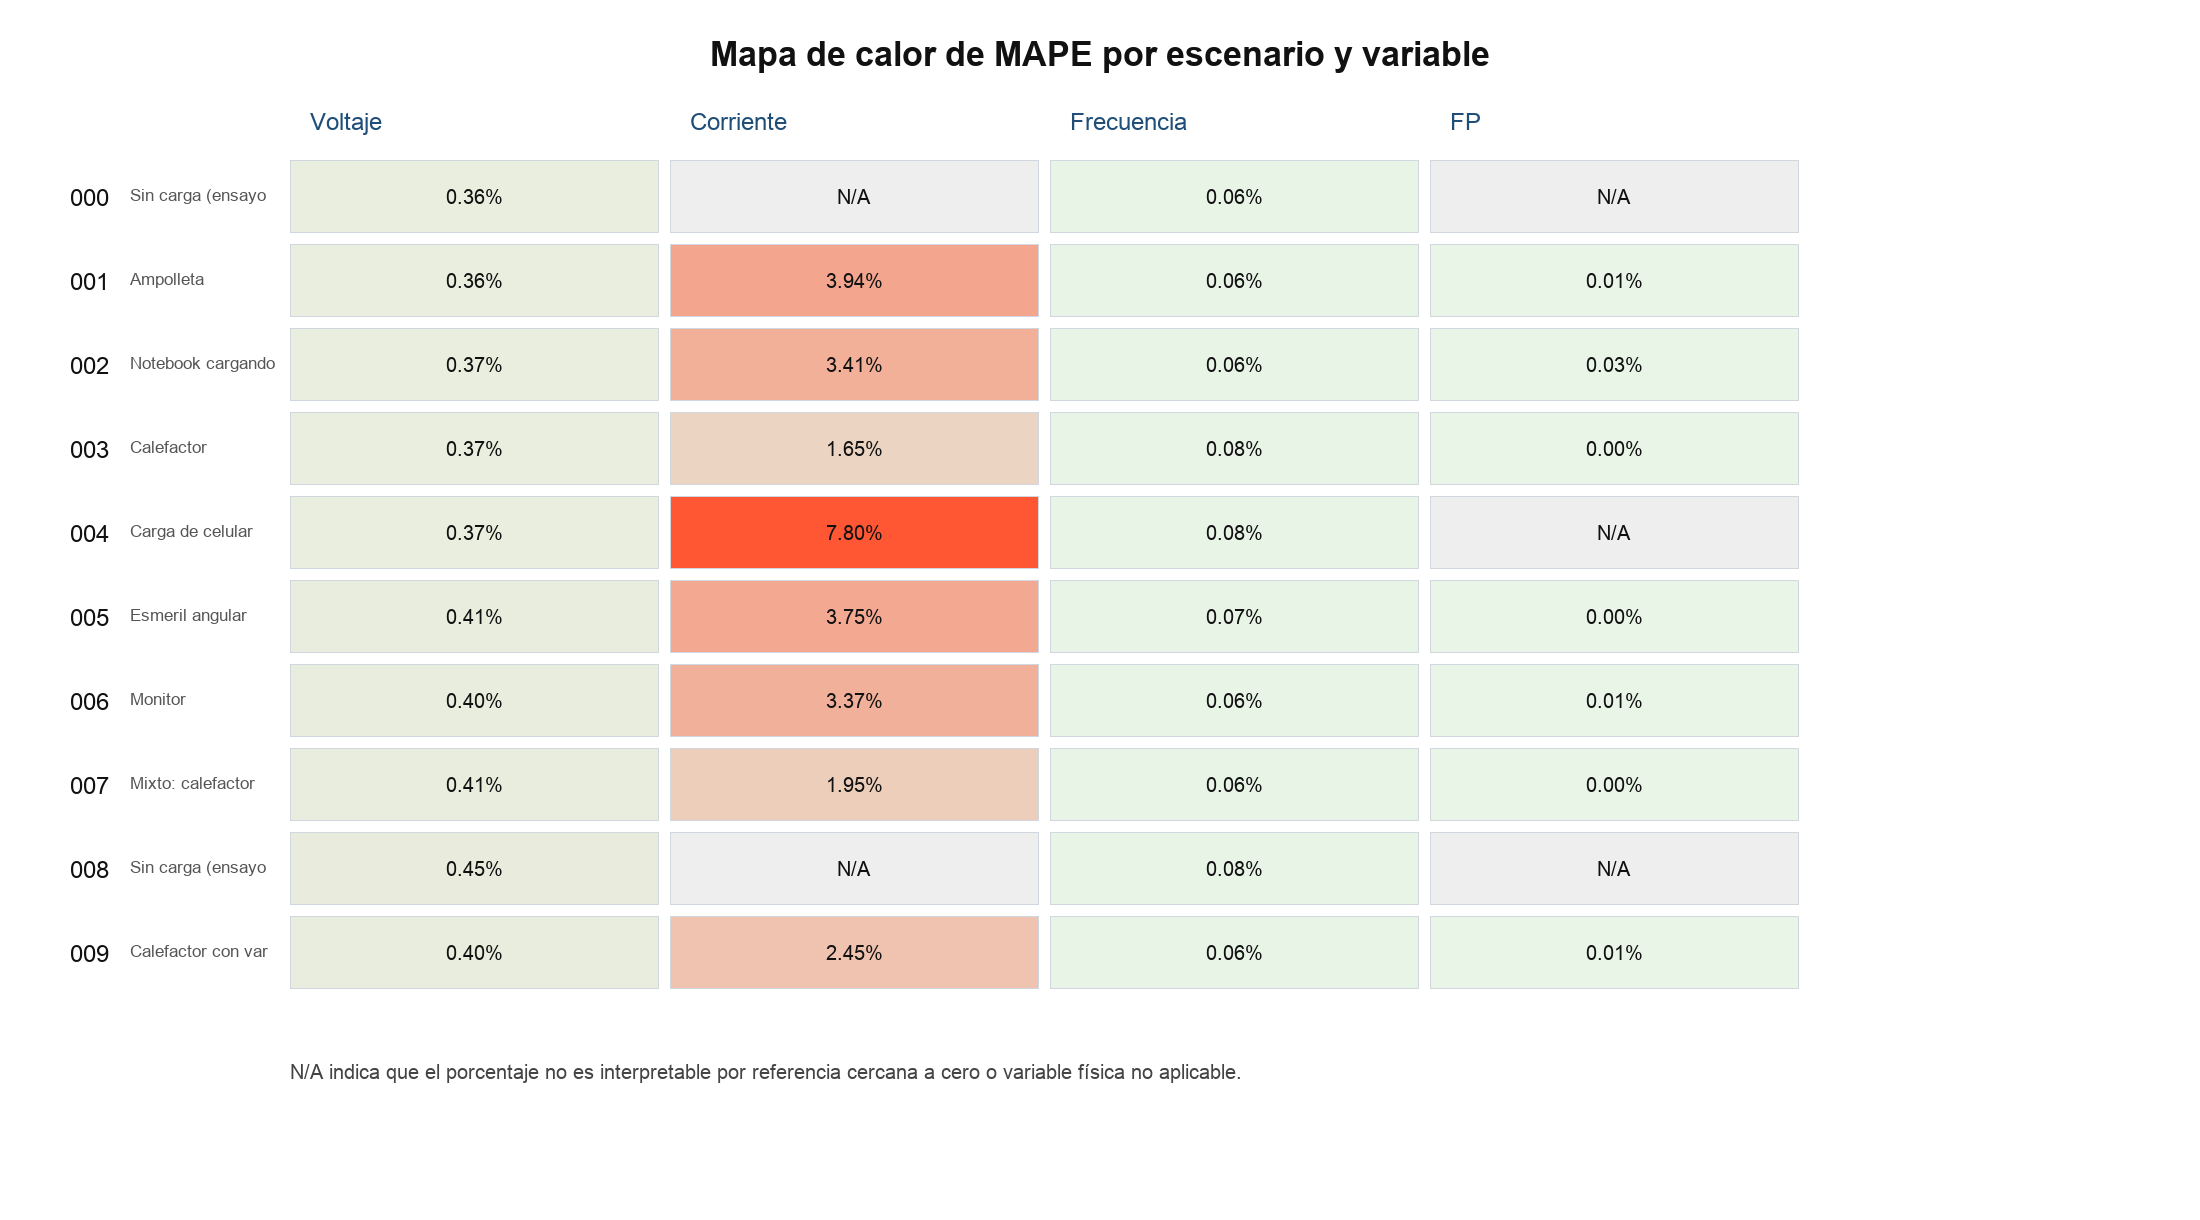
\includegraphics[width=0.92\textwidth]{figures/image8.png}
\caption{MAPE heat map by scenario and variable. The scale highlights where relative error increases due to low load or operational variability.}
\label{fig:8}
\end{figure*}

Figure~\ref{fig:8} shows that voltage remains stable across scenarios, with MAPE between 0.36\% and 0.45\%. This indicates that EnPi voltage measurement is consistent for operational monitoring in the tested 220--230 V single-phase networks. For current, relative error increases at low loads, especially for mobile phone charging, where MAE is low in absolute terms but the reference denominator is also small. Therefore, current interpretation is separated between no-load or low-load conditions, where MAE is more informative, and productive or thermal load conditions, where MAPE enables proportional error comparison.

\begin{table*}[t]
\caption{Global correlation and Bland-Altman agreement between EnPi and Metrel MI2883.}
\label{tab:correlacion-global-y-acuerdo-de-bland-altman-}
\centering
\scriptsize
\begin{adjustbox}{max width=\textwidth}
\begin{tabular}{ccccccc}
\toprule
Variable & Pearson r & R\textasciicircum{}2 & Bias & SD & Lower LoA & Upper LoA \\
\midrule
Voltage & 0.9840 & 0.9682 & 0.8947 & 0.2994 & 0.3079 & 1.4815 \\
Current & 0.9998 & 0.9997 & -0.0589 & 0.0835 & -0.2225 & 0.1048 \\
Frequency & 0.8255 & 0.6815 & -0.0410 & 0.0532 & -0.1452 & 0.0633 \\
Power factor & 0.9987 & 0.9974 & -0.0009 & 0.0131 & -0.0265 & 0.0247 \\
\bottomrule
\end{tabular}
\end{adjustbox}
\end{table*}

\begin{figure*}[!t]
\centering
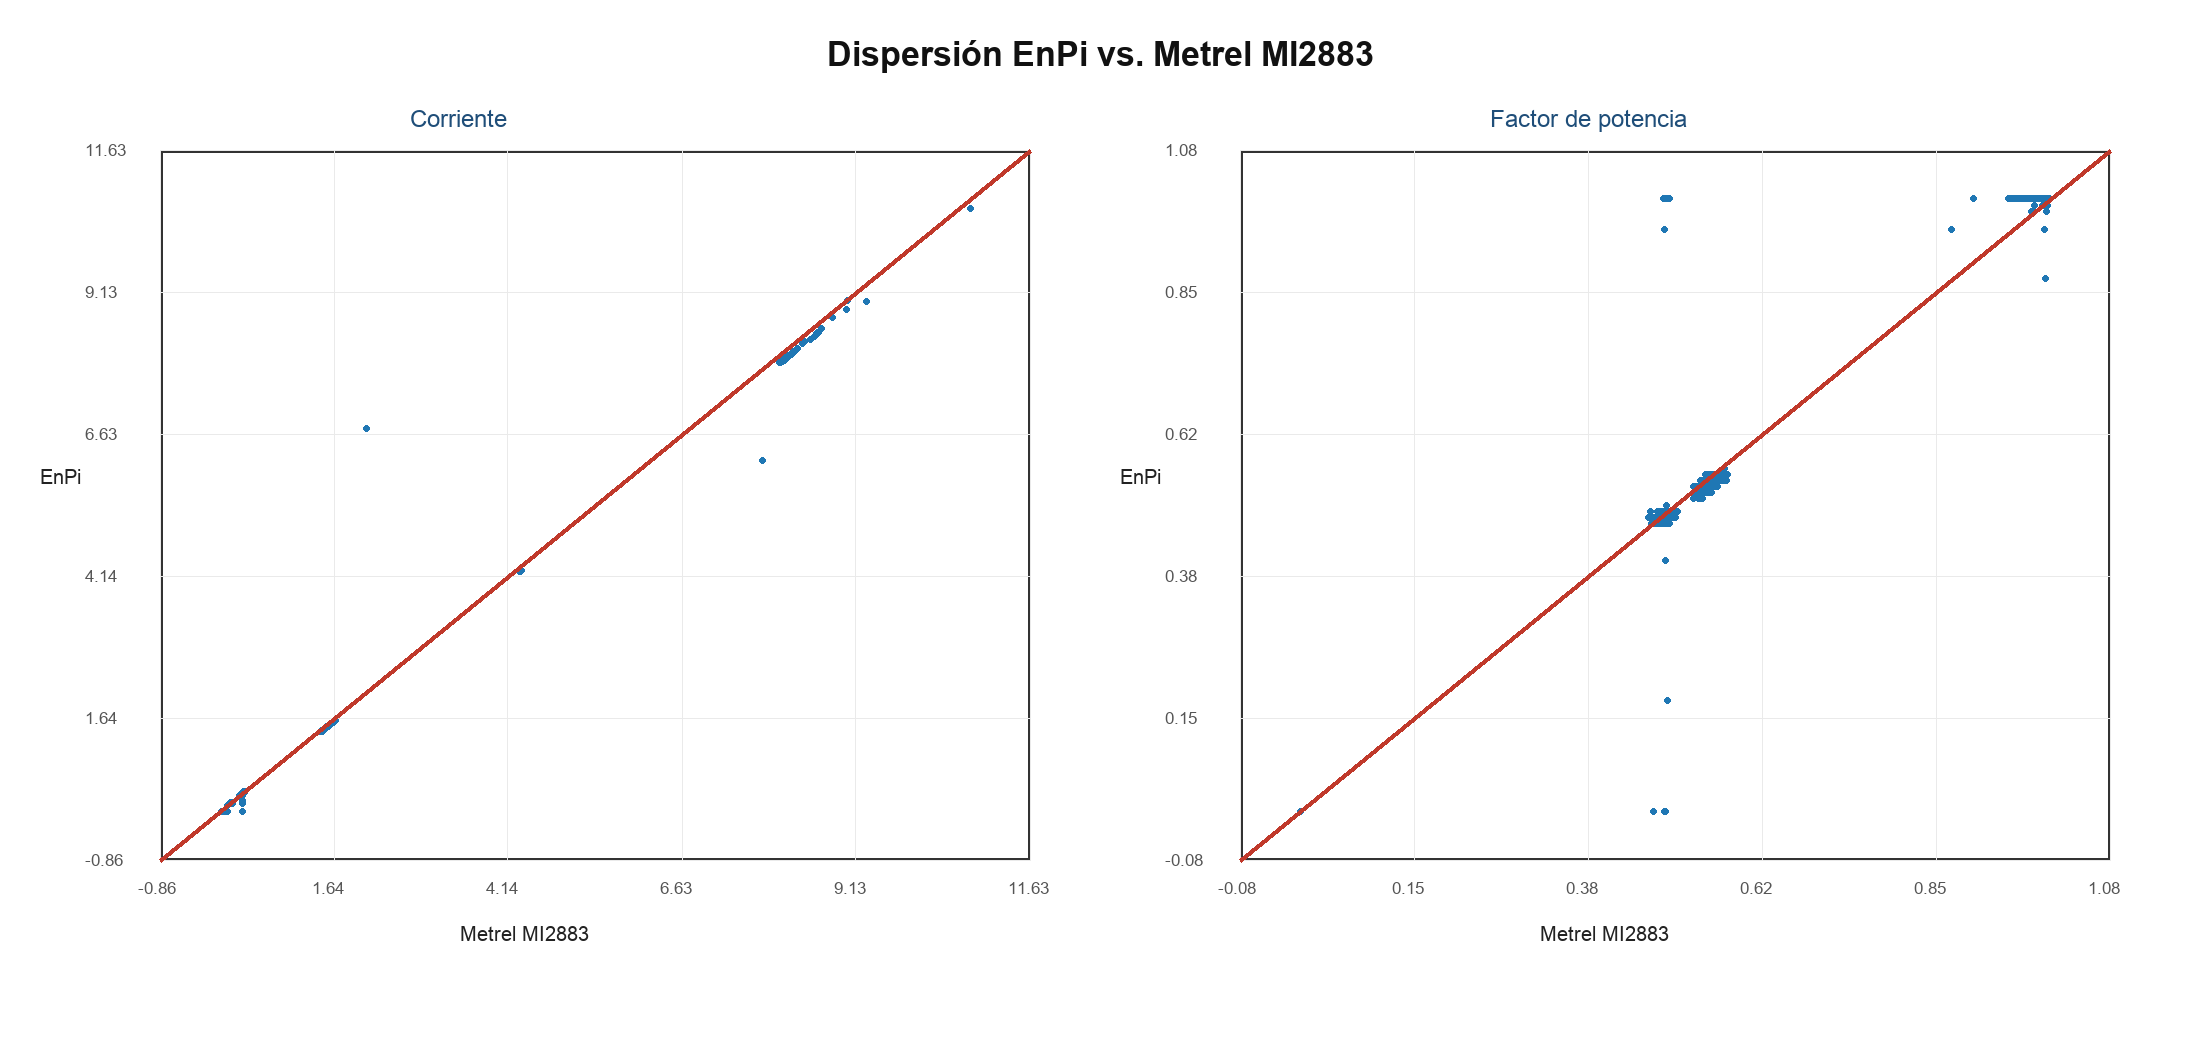
\includegraphics[width=\textwidth]{figures/image9.png}
\caption{EnPi-Metrel scatter plot for current and power factor. The red line represents ideal agreement, y=x.}
\label{fig:9}
\end{figure*}

Figure~\ref{fig:9} evaluates whether the system preserves proportionality with respect to the reference instrument. Current shows nearly linear alignment, consistent with r=0.9998 and R\textasciicircum{}2=0.9997. This evidence must be interpreted together with absolute errors and limits of agreement, because high correlation alone does not imply metrological agreement. Power factor also shows high global agreement, with r=0.9987 and R\textasciicircum{}2=0.9974, supporting the preliminary use of EnPi to characterize resistive, electronic, inductive, or mixed profiles in energy-management analysis.

\begin{figure*}[!t]
\centering
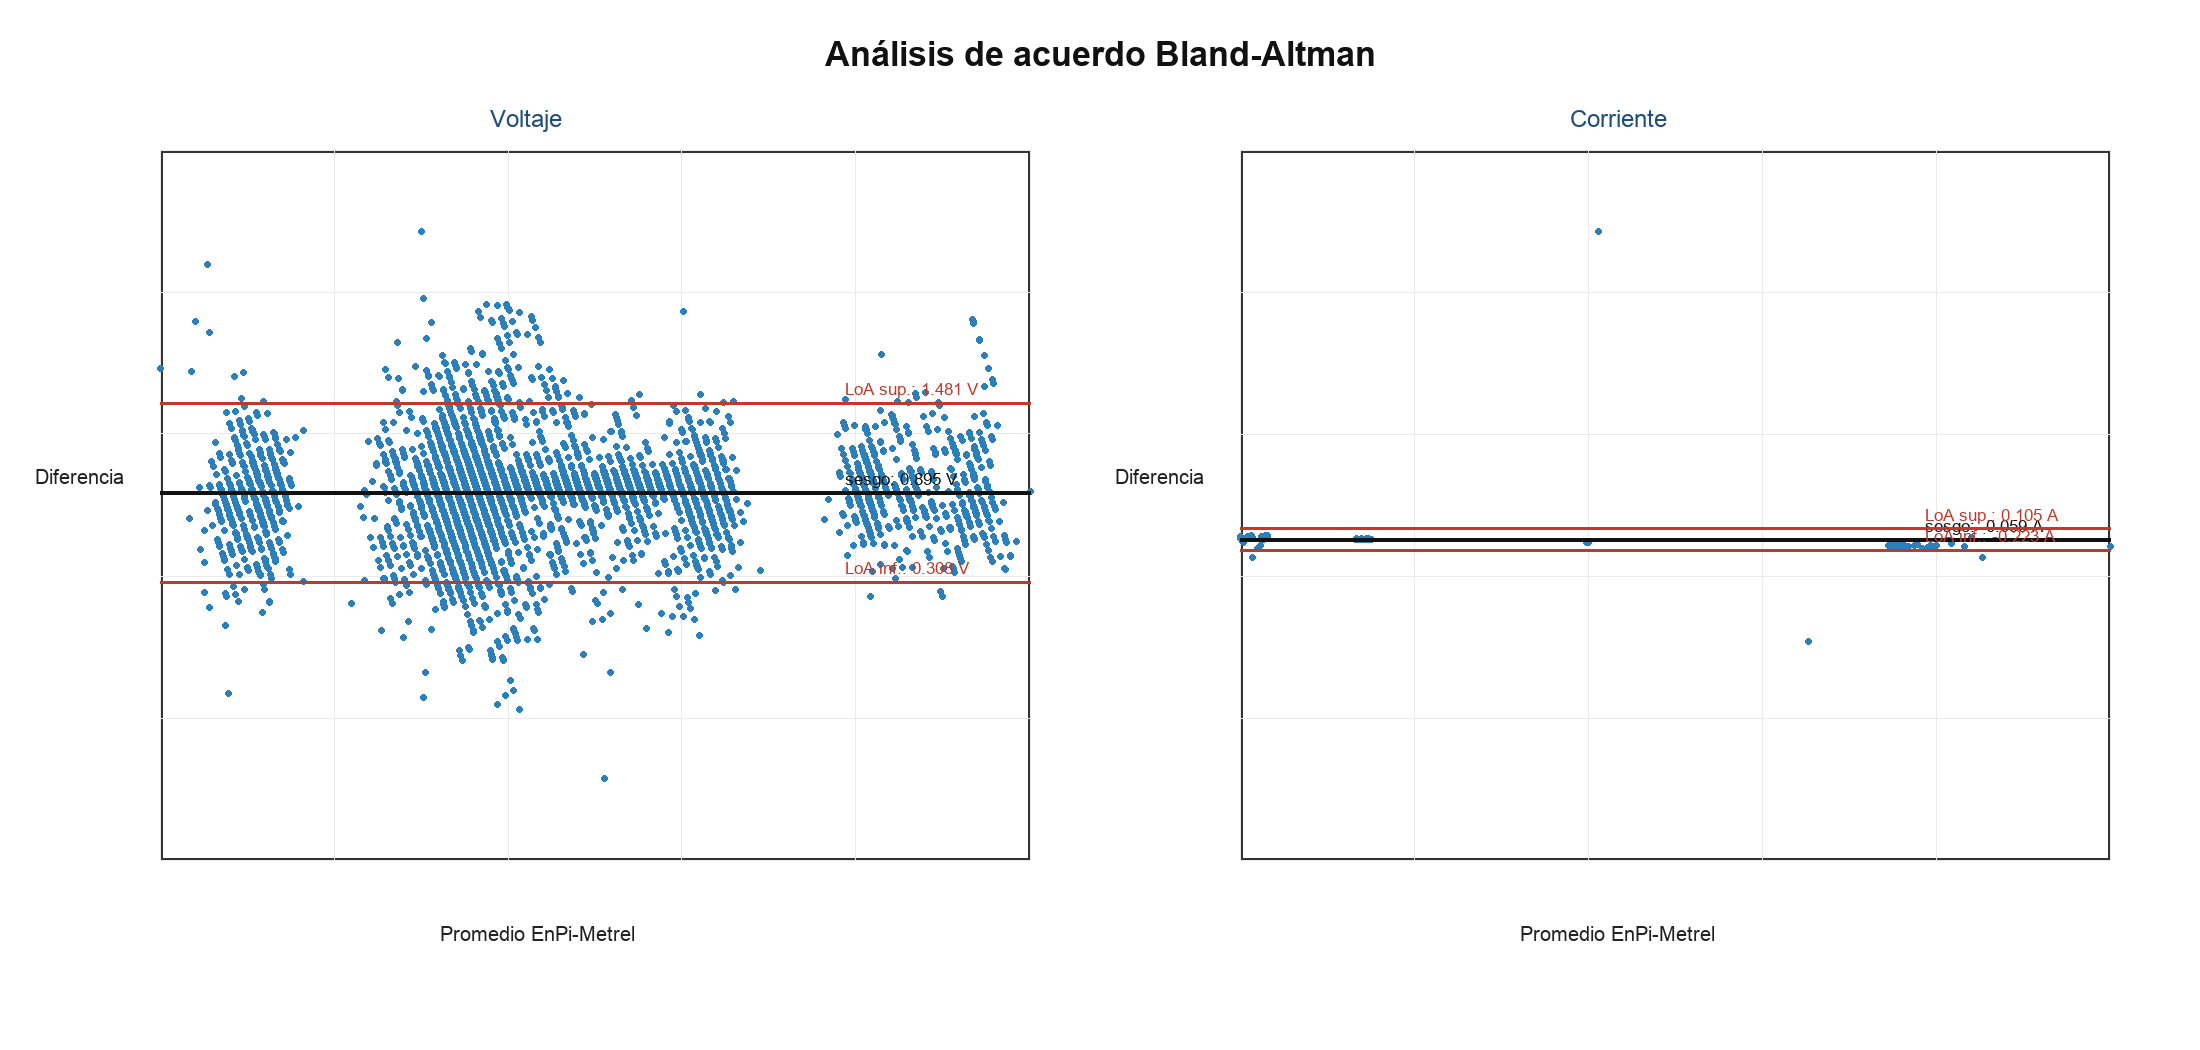
\includegraphics[width=0.92\textwidth]{figures/image10.png}
\caption{Bland-Altman analysis for voltage and current. Horizontal lines show mean bias and 95\% limits of agreement.}
\label{fig:10}
\end{figure*}

Figure~\ref{fig:10} complements the correlation analysis by showing agreement in physical units. For voltage, the mean bias is approximately 0.895 V, with limits of agreement between 0.308 V and 1.481 V. This suggests a small systematic difference, compatible with an instrumental offset and potentially correctable through secondary calibration if greater accuracy is required. For current, the mean bias is -0.0589 A, with limits of agreement between -0.2225 A and 0.1048 A; therefore, EnPi tends to slightly underestimate relative to Metrel. For operational equipment-level monitoring, this magnitude is acceptable within the tested range and the criteria in Table~\ref{tab:criterios-operacionales}, but it should be declared if the system is used for high-precision energy balances.

\begin{table*}[!t]
\caption{Active power estimated from Metrel variables and exploratory comparison with EnPi power.}
\label{tab:potencia-activa-estimada-a-partir-de-variable}
\centering
\scriptsize
\begin{adjustbox}{max width=\textwidth}
\begin{tabular}{ccccc}
\toprule
Sc. & n & MAE kW & RMSE kW & MAPE \\
\midrule
000 & N/A & N/A & N/A & N/A \\
001 & 1202 & 0.0017 & 0.0019 & 2.67\% \\
002 & 1191 & 0.0015 & 0.0030 & 4.04\% \\
003 & 900 & 0.0240 & 0.0242 & 1.31\% \\
004 & N/A & N/A & N/A & N/A \\
005 & 1201 & 0.0098 & 0.0098 & 2.94\% \\
006 & 1201 & 0.0023 & 0.0023 & 5.22\% \\
007 & 1181 & 0.0310 & 0.0310 & 1.59\% \\
008 & 900 & 0.0000 & 0.0000 & N/A \\
009 & 1040 & 0.0245 & 0.0501 & 2.08\% \\
\bottomrule
\end{tabular}
\end{adjustbox}
\end{table*}

Active power is reported as an exploratory analysis because the consolidated file did not include a direct active-power column exported from Metrel. The reference was calculated as P = U$\cdot$I$\cdot$PF using voltage, corrected current, and Metrel power factor. For this reason, the active-power comparison is interpreted as an energy-consistency check rather than as a direct metrological validation of that variable.

\subsection{Technical Discussion of Results}
\label{subsec:technical-discussion}

The results support the central thesis of the article: EnPi is not intended to replace a calibrated power quality analyzer, but to provide a distributed, low-cost, and traceable layer for equipment-level energy monitoring. Under this definition of use, the observed performance is solid. Voltage shows low absolute error, current maintains high linearity in the range of greater energy-management interest, power factor preserves high global agreement, and frequency shows small absolute errors.

The main weakness appears at low currents and no-load scenarios. This does not invalidate the system; rather, it defines its boundary of use. Under standby or small-load conditions, MAE should be prioritized over MAPE because percentages may be artificially amplified. Under production, heating, tool, or combined-equipment loads, relative error improves and becomes more useful for management decisions.

Methodologically, the control of unpaired records is a strength of the study. If two instruments are aligned by timestamp rounded to the second, one sample taken at the beginning of a second and another at the end may be separated by almost a full second. Under variable loads, this introduces artificial error. Therefore, documenting packet losses, excluding unpaired records, and preserving continuous segments improve the internal validity of the experiment. The subsequent firmware modification to store and re-inject readings under intermittent connectivity should be understood as an operational-continuity improvement for future campaigns, not as reprocessing of the already reported experimental evidence.

In summary, the comparison with the calibrated Metrel MI2883 provides defensible preliminary evidence for the single-phase metering component. The evidence does not legally certify the device or validate the full industrial platform by itself, but supports its use as an operational IoT node within the tested range for traceability, consumption-pattern detection, initial prioritization of metering points, and support for EnPI calculation.

\section{Discussion}
\label{sec:discussion}

The inclusion of parallel measurement changes the scope of the work: EnPi is no longer presented only as a conceptual architecture, but also includes preliminary quantitative evidence on the performance of the single-phase node. However, this evidence validates the acquisition component under controlled scenarios, not the complete SaaS-IoT platform in industrial operation. The SaaS contribution should therefore be interpreted as an implemented traceability and EnPI-calculation workflow, while the quantitative validation should be interpreted as evidence for the tested metering component and its ability to feed that workflow under the reported conditions. Comparison with a calibrated analyzer makes it possible to estimate measurement error and discuss the node's limits, while long-term operational continuity and plant-level usefulness must be evaluated in future industrial campaigns.

The main difference between EnPi and works focused only on smart metering is its progressive adoption approach. A company can begin with manual data and billing records, obtain an initial baseline, define indicators, and later incorporate IoT metering where it adds value. This design recognizes that many organizations do not begin from an instrumented plant, but from incomplete information and dispersed administrative processes.

The use of EnPI as the central indicator strengthens the contribution by shifting the analysis from absolute consumption to productive energy performance. This allows periods, machines, or work centers to be compared even when production changes, provided that the production unit and period are consistent. The anonymized real case in a food-sector SME demonstrates this logic in a dough sheeter by linking corrected IoT readings, daily energy, and declared production of 44 kg of dough per production day across a 17-day operational period. The observed values were within a range compatible with published references for kneading and dough-preparation operations in bakeries, although these comparisons should be understood as operational benchmarks rather than universal normative criteria [22], [23].

The operational value of the case is not limited to reporting a daily kWh/kg value. The dashboard and alert rules transformed the EnPI series into a practical diagnostic trigger: four days were classified as critical, with deviations from +33.67\% to +59.99\% relative to the reference. This evidence enabled the business owner to examine possible causes of abnormal energy intensity using local operational knowledge. From a methodological perspective, this is important because the platform does not claim to infer causality from electrical measurements alone. Instead, it organizes time-stamped consumption, production, reference, deviation, and status information so that human operators can investigate plausible causes such as differences in machine use, number of dough passes, idle operation, cleaning routines, scheduling, or effective load. This positions EnPi as a decision-support and traceability tool rather than an autonomous diagnostic system.

The limitations are relevant. Initial validation at a single-phase point does not, by itself, represent industrial environments with high-power motors, three-phase loads, variable frequency drives, transients, or electrical noise. The food-sector SME case provides a real demonstration of EnPI traceability and alert-based follow-up, but it does not constitute multi-company statistical validation and does not isolate all operational factors that may affect specific consumption. The production denominator was declared as a constant daily quantity, and the analysis did not independently measure dough type, number of passes, effective load, waiting times, cleaning periods, or intermittent equipment use. Nor does it demonstrate simultaneous performance of multiple nodes or long-term robustness under intermittent connectivity. Therefore, a higher-current single-phase variant and a three-phase panel version may be incorporated as scalability extensions, but the initial experimental contribution should remain centered on demonstrating preliminary accuracy within the validated range and operational traceability in a bounded use case.

\section{Conclusions and Future Work}
\label{sec:conclusions}

This work presents EnPi, a modular SaaS-IoT platform for progressive adoption of industrial energy management, whose analytical core is the calculation of EnPI indicators from energy consumed and production obtained. The proposal integrates a data model, manual records, IoT readings, target references, traceability, reconciliation, and visualization of deviations. The evidence reported in this article supports two bounded claims: first, that the implemented SaaS workflow can organize traceable energy, production, and indicator records; and second, that the tested single-phase node can provide preliminary operational measurements compatible with that workflow under the evaluated scenarios. The article also incorporates preliminary experimental validation of the single-phase node through parallel measurements against a calibrated Metrel MI2883 power quality analyzer and an anonymized real EnPI traceability case in a food-sector SME dough sheeter.

The results support the use of EnPi as an operational monitoring and traceability tool under the tested single-phase conditions, but they do not certify the device or validate the complete platform in real industrial environments. Future work will extend the experimental validation toward longer campaigns, real industrial scenarios, three-phase metering, higher-current versions, simultaneous deployment of multiple nodes, and direct comparison of active power and accumulated energy exported from reference instruments. Future work should also deepen cybersecurity mechanisms, access control, remote firmware management, resilience under intermittent connectivity, acceptance by industrial users, and validation of EnPI indicators in more companies, products, and production conditions.

\section*{Acknowledgment}
This work was supported by the Centre for Innovation in Technology and Design of Materials for the Built Environment (CIMAC), ANID CTI250005.

\section*{Data and Code Availability}

The raw data and processed data supporting the reported EnPi--Metrel comparison and operational EnPI case are publicly available in the EnPi repository: \url{https://github.com/The-Terial/Enpi}. The repository should be used as the primary source for reproducing the reported tables, figures, exclusion criteria, and calculation workflow. The node firmware is identified by version in this manuscript; if full firmware disclosure is restricted by project policy, the corresponding version identifier or hash should be retained to preserve auditability.

\begin{thebibliography}{99}
\bibitem{ref1} M. U. Saleem, M. R. Usman, and M. Shakir, "Design, Implementation, and Deployment of an IoT Based Smart Energy Management System," IEEE Access, vol. 9, pp. 59649-59664, 2021, doi: 10.1109/ACCESS.2021.3070960.
\bibitem{ref2} M. Ullah, A. Narayanan, A. Wolff, and P. H. J. Nardelli, "Industrial Energy Management System: Design of a Conceptual Framework Using IoT and Big Data," IEEE Access, vol. 10, pp. 110557--110567, 2022, doi: 10.1109/ACCESS.2022.3215167.
\bibitem{ref3} Y. Li, Z. Sun, L. Han, and N. Mei, "Fuzzy Comprehensive Evaluation Method for Energy Management Systems Based on an Internet of Things," IEEE Access, vol. 5, pp. 21312-21322, 2017, doi: 10.1109/ACCESS.2017.2728081.
\bibitem{ref4} M. U. Saleem, M. R. Usman, M. A. Yaqub, A. Liotta, and A. Asim, "Smarter Grid in the 5G Era: Integrating the Internet of Things With a Cyber-Physical System," IEEE Access, vol. 12, pp. 34002--34018, 2024, doi: 10.1109/ACCESS.2024.3372379.
\bibitem{ref5} S. Kim, S. Lee, M. Kim, and Y. Kwon, "A Web Application Framework for Battery Health Prediction in Industrial IoT Networks," Journal of Web Engineering, vol. 24, no. 6, pp. 943-972, 2025, doi: 10.13052/jwe1540-9589.2464.
\bibitem{ref6} S. M. A. A. Abir, A. Anwar, J. Choi, and A. S. M. Kayes, "IoT-Enabled Smart Energy Grid: Applications and Challenges," IEEE Access, vol. 9, pp. 50961-50981, 2021, doi: 10.1109/ACCESS.2021.3067331.
\bibitem{ref7} Y. Santo, A. Abelem, A. Riker, and E. E. Tsiropoulou, "Integrating Data Privacy and Energy Management in Smart Cities With Partial Sustainable IoT Networks," IEEE Access, vol. 13, pp. 33176--33188, 2025, doi: 10.1109/ACCESS.2025.3541213.
\bibitem{ref8} O. Said, Z. Al-Makhadmeh, and A. Tolba, "EMS: An Energy Management Scheme for Green IoT Environments," IEEE Access, vol. 8, pp. 44983-44998, 2020, doi: 10.1109/ACCESS.2020.2976641.
\bibitem{ref9} B. Safaei, M. Peiravian, and M. Siamaki, "Eco-Friendly IoT: Leveraging Energy Harvesting for a Sustainable Future," IEEE Sensors Reviews, vol. 2, pp. 32--75, 2025, doi: 10.1109/SR.2025.3552043.
\bibitem{ref10} L. N. H. Pham, A. Shrestha, C. Sharma, and F. Gonzalez-Longatt, "Digital Twins and Cyber-Physical Systems Toward the Digitalization of Power and Energy Systems," IEEE Transactions on Technology and Society, vol. 6, no. 4, pp. 393--410, 2025, doi: 10.1109/TTS.2025.3615624.
\bibitem{ref11} M. S. Ahmad et al., "Demand Response Program Toward Sustainable Power Supply: Current Status, Challenges, and Prospects in Malaysia," IEEE Access, vol. 13, pp. 34706--34731, 2025, doi: 10.1109/ACCESS.2025.3541841.
\bibitem{ref12} K. Shafique, B. A. Khawaja, F. Sabir, S. Qazi, and M. Mustaqim, "Internet of Things (IoT) for Next-Generation Smart Systems: A Review of Current Challenges, Future Trends and Prospects for Emerging 5G-IoT Scenarios," IEEE Access, vol. 8, pp. 23022-23040, 2020, doi: 10.1109/ACCESS.2020.2970118.
\bibitem{ref13} J. S. Yalli, M. H. Hasan, and A. A. Badawi, "Internet of Things (IoT): Origins, Embedded Technologies, Smart Applications, and Its Growth in the Last Decade," IEEE Access, vol. 12, pp. 91357--91382, 2024, doi: 10.1109/ACCESS.2024.3418995.
\bibitem{ref14} M. Soula, B. Mbarek, and A. Meddeb, "A Real-Time Trust Management Model Using Digital Twin in IoT Networks," IEEE Access, vol. 12, pp. 183326--183343, 2024, doi: 10.1109/ACCESS.2024.3506870.
\bibitem{ref15} A. Bounceur et al., "Phygital Twin IoT: A Hardware-Software Decomposition Architecture for Scalable and Secure Digital Twin IoT Systems," IEEE Open Journal of the Computer Society, vol. 7, pp. 755--768, 2026, doi: 10.1109/OJCS.2026.3681725.
\bibitem{ref16} A. Velez-Estevez, L. Gutierrez-Madronal, and I. Medina-Bulo, "IoT-TEG 4.0: A New Approach 4.0 for Test Event Generation," IEEE Transactions on Reliability, vol. 71, no. 3, pp. 1368--1380, 2022, doi: 10.1109/TR.2021.3087781.
\bibitem{ref17} M. S. Yaraziz and R. Hill, "Federated Q-Learning-Based Optimization for Resource Allocation in Industrial IoT Networks," IEEE Access, vol. 13, pp. 188880--188891, 2025, doi: 10.1109/ACCESS.2025.3624919.
\bibitem{ref18} H. Zhu, K. Ouahada, and A. M. Abu-Mahfouz, "Peer-to-Peer Energy Trading in Smart Energy Communities: A Lyapunov-Based Energy Control and Trading System," IEEE Access, vol. 10, pp. 42916--42932, 2022, doi: 10.1109/ACCESS.2022.3167828.
\bibitem{ref19} International Organization for Standardization, ISO 50001:2018, Energy management systems --- Requirements with guidance for use, Geneva, Switzerland: ISO, 2018.
\bibitem{ref20} International Organization for Standardization, ISO 50006:2023, Energy management systems --- Evaluating energy performance using energy performance indicators and energy baselines, Geneva, Switzerland: ISO, 2023.
\bibitem{ref21} G. W. Hart, ``Nonintrusive Appliance Load Monitoring,'' Proceedings of the IEEE, vol. 80, no. 12, pp. 1870--1891, Dec. 1992, doi: 10.1109/5.192069.
\bibitem{ref22} M. Briceño-León, D. Pazmiño-Quishpe, J.-M. Clairand, and G. Escrivá-Escrivá, ``Energy Efficiency Measures in Bakeries toward Competitiveness and Sustainability--Case Studies in Quito, Ecuador,'' Sustainability, vol. 13, no. 9, Art. no. 5209, 2021, doi: 10.3390/su13095209.
\bibitem{ref23} F. Paschino and F. Gambella, ``Comparison between traditional and industrial plants used for production of `carasau' bread and evaluation of final products,'' Applied Engineering in Agriculture, vol. 23, no. 1, pp. 65--70, 2007, doi: 10.13031/2013.22319.
\bibitem{ref24} J. Varela-Aldás, S. Silva, and G. Palacios-Navarro, ``IoT-Based Alternating Current Electrical Parameters Monitoring System,'' Energies, vol. 15, no. 18, Art. no. 6637, 2022, doi: 10.3390/en15186637.
\bibitem{ref25} International Electrotechnical Commission, IEC 62053-21:2020, Electricity metering equipment --- Particular requirements --- Part 21: Static meters for AC active energy (classes 0,5, 1 and 2), Geneva, Switzerland: IEC, 2020.
\end{thebibliography}

\begin{IEEEbiography}[{
\includegraphics[width=1in,height=1.25in,clip,keepaspectratio]{figures/andres_viveros_bio.png}}]{Andres Viveros}
Andres Viveros received the Industrial Civil Engineering degree, the M.B.A. degree, and the Ph.D. degree from the University of Santiago of Chile (USACH), Chile. He has professional experience in operations, management control, business intelligence, process redesign, change management, and project management. He has 15 years of teaching experience in production and enterprise resource planning systems. His professional and research interests include operational transformation, digital ecosystems, energy management systems, IoT-based monitoring, energy performance indicators, and traceable digital platforms for industrial and small- and medium-sized enterprise environments.
\end{IEEEbiography}

\begin{IEEEbiography}[{
\includegraphics[width=1in,height=1.25in,clip,keepaspectratio]{figures/ivan_derpich_bio.jpg}}]{Ivan Derpich}
Dr. Ivan Derpich, Professor of the Department of Industrial Engineering at the University of Santiago de Chile. Industrial Civil Engineer from the University of Santiago de Chile and Ph.D. in Engineering Sciences, mention in Industrial Engineering, from the Catholic University of Chile. He has been a consultant for companies and has been Director of the Master in Industrial Engineering and Director of the Doctorate in Engineering, mention in Industrial Engineering, at the same university. Member of the Chilean Institute of Operations Research (ICHIO). He has developed research in operations research, in particular integer linear programming.He is the author of nearly 40 research articles and is currently the principal investigator for the circular logistics research line at a research center specializing in materials and circular logistics.
\end{IEEEbiography}

\begin{IEEEbiography}[{
\includegraphics[width=1in,height=1.25in,clip,keepaspectratio]{figures/juan_sepulveda_bio.jpg}}]{Juan Miguel Sepulveda}
Juan Sepulveda received the Industrial Civil Engineering degree from the University of Santiago of Chile (USACH), Chile, and the M.Sc. and Ph.D. degrees in Engineering Science, with a focus on Industrial and Systems Engineering, from The University of Tennessee, Knoxville, USA. He is a Full Professor with the Department of Industrial Engineering, University of Santiago of Chile. His research interests include supply chain management, humanitarian logistics and disaster response, complex systems modeling in manufacturing and mining, Industry 5.0, computational intelligence, and sustainable production systems. He has also held several academic leadership positions at USACH, including roles related to graduate programs and the Department of Industrial Engineering.
\end{IEEEbiography}

\EOD

\end{document}
